% File project.tex
%% Style files for ACL 2021
\documentclass[11pt,a4paper]{article}
\usepackage[hyperref]{acl2021}
\usepackage{times}
\usepackage{booktabs}
\usepackage[draft]{todonotes}
\usepackage{latexsym}
% \usepackage[demo]{graphicx}
\usepackage{subcaption}
\usepackage[title]{appendix}
\usepackage{float}
\usepackage{amsmath}
\usepackage{amsfonts}
\usepackage{indentfirst}
\usepackage{xcolor}
\usepackage{natbib, multirow}
\usepackage{graphics}
\usetikzlibrary{shapes.geometric}


% \usepackage{subfig}
\renewcommand{\UrlFont}{\ttfamily\small}


% Packages for collaborative annotations
\usepackage{comment}
%\usepackage[draft]{todonotes}
% This is not strictly necessary, and may be commented out,
% but it will improve the layout of the manuscript,
% and will typically save some space.
\usepackage{microtype}

\aclfinalcopy 

\newcommand\BibTeX{B\textsc{ib}\TeX}

\title{Improving Action Segmentation on Large Egocentric Cooking Dataset}

\author{
  Yun Cheng\thanks{\hspace{4pt}Everyone Contributed Equally -- Alphabetical order} \hspace{2em} Yuxuan Liu$^*$ \hspace{2em} Tiffany Ma$^*$ \hspace{2em} Erin Zhang$^*$ \\
  \texttt{\{yuncheng, yuxuanli, tma1, xiaoyuz1\}@andrew.cmu.edu}
}

\date{\today}

\begin{document}
\maketitle
\begin{abstract}
The task of action segmentation involves identifying not only the start and end time of different actions in an untrimmed video but also the action types. Previous approaches take in only visual inputs, whereas we attempt to solve the task using additional text input. We test our methods on the EPIC-KITCHENS dataset, whose narration annotations allow us to learn a visual-textual joint-embedding. We build upon the existing MS-TCN model which produces the start and end time of segments in a video, and we uses the visual features of the predicted segment to retrieve the closest narration in terms of their distance in the joint space. Although the video-text retrieval component does not improve baseline performance, we analyze its strength in terms of action recognition and the causes of potential failure cases. 
\end{abstract}

\section{Introduction and Problem Definition}

Localizing and classifying activities in long untrimmed video is of great importance in video understanding ranging from video indexing to surveillance and robotics. Action segmentation is a video understanding task about identifying when and what type of action in a given video. This is done by temporally locating action segments in the video and classifying the action category of each segment. To capture long-range dependencies of action events in long untrimmed videos, recent methods using dilated temporal convolutions \cite{8953830,9186840} and dilated temporal graphs for temporal reasoning \cite{graphbased2020,wang2020temporal} have been very successful. While they can achieve decent performance on less complex datasets \cite{Ishikawa_2021_WACV}, the performance significantly drops when the models are evaluated on large, challenging datasets as indicated by \newcite{graphbased2020}. We see there is still room for performance improvement due to the inherent complexity of the task and the dataset.


\begin{figure}[t]
    \centering
    \begin{tikzpicture}[scale=0.7]
        \node[] at (4,-8) {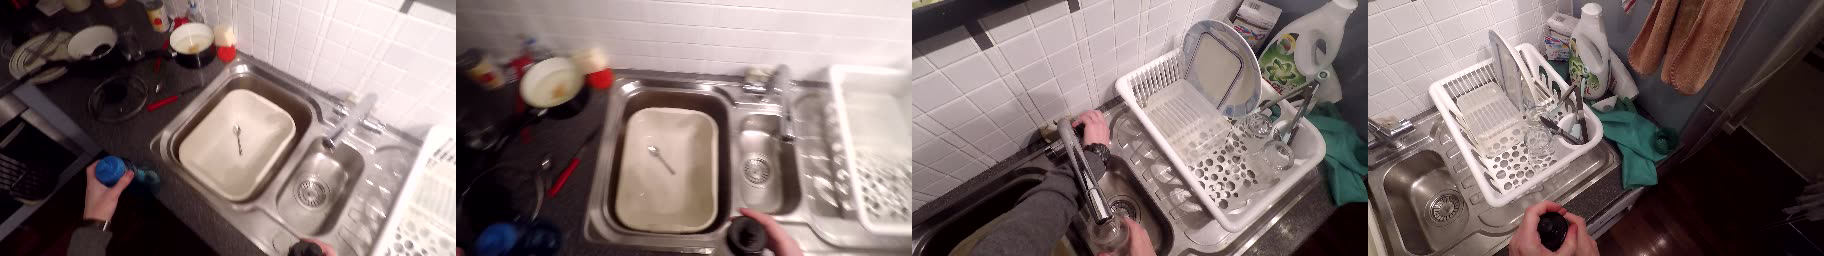
\includegraphics[scale=0.1]{figures/input.png}};
        \draw[->,-stealth,semithick] (4,-7.6) to (4,-6.5);
        
        \filldraw[fill=black!5!white,rounded corners=5] (2,-6.5) rectangle (6,-5.5) node[pos=0.5] {\small SS-TCN Stage 1};
        \draw[->,-stealth,densely dashed,semithick] (4,-5.5) to (4,-4.5);
        \filldraw[fill=black!5!white,rounded corners=5] (2,-4.5) rectangle (6,-3.5) node[pos=0.5] {\small SS-TCN Stage 4};
        \draw[rounded corners=5,densely dashed] (0,-7) rectangle (8,-3);
        \node[] at (7,-5) {\textbf{\textsf{\scriptsize Backbone}}};
        \draw[->,-stealth,semithick] (4,-3.5) to (4,-2.4);
        \filldraw[fill=red!40!white, draw=black] (0,-2.4) rectangle (2.5,-2);
        \filldraw[fill=cyan!40!white, draw=black] (2.5,-2.4) rectangle (6.5,-2);
        \filldraw[fill=blue!40!white, draw=black] (6.5,-2.4) rectangle (8,-2);
        \draw[] (0,-2.4) rectangle (8,-2) node[pos=0.5] {\small Prediction};

        \filldraw[fill=red!40!white, draw=black] (0,4) rectangle (2.5,4.4);
        \filldraw[fill=yellow!40!white, draw=black] (2.5,4) rectangle (6.5,4.4);
        \filldraw[fill=green!40!white, draw=black] (6.5,4) rectangle (8,4.4);
        \draw[] (0,4) rectangle (8,4.4) node[pos=0.5] {\small Prediction};
        \draw[->,-stealth,semithick] (4,-2) to (4,4);
        \filldraw[fill=black!5!white,rounded corners=5] (-0.5,0) rectangle (2.5,2) node[text width=2cm,pos=0.5,align=center] {\small Video-to-Text Retrieval};
        \filldraw[fill=black!20!white, draw=black] (-1.6,-1) rectangle (0.4,-0.5) node[pos=0.5] {\footnotesize Narrations};
        \draw[->,-stealth,semithick] (0.4,-0.75) -- (0.8,-0.75) -- (0.8,0);
        \draw[->,-stealth,semithick] (4,-0.75) -- (1.2,-0.75) -- (1.2,0);
        \draw[->,-stealth,semithick] (1,2) -- (1,2.5) -- (4,2.5);
        \draw[rounded corners=5,densely dashed] (-1.7,-1.5) rectangle (8,3.5);
        \node[text width=2.5cm, align=center] at (6,1) {\textbf{\textsf{\scriptsize Video-Text Retrieval Module}}};
    \end{tikzpicture}
    \caption{Overview of the proposed approach. The backbone model is MS-TCN, which is a stack of four single-stage TCNs (SS-TCN). Our video-text retrieval module extracts segments from the initial segmentation predicted by the backbone and retrieves the most relevant narration of each segment. Then the frame-wise classification label are updated with the verb in the retrieved narration.}
    \label{fig:overview-of-appraoch}
\end{figure}

There are two sub-challenges in action segementation, namely 1) localizing the events for action segments and 2) classifying the action in each segment. While the two sub-challenges are highly dependent on each other, we empirically found that misclassification is a more prominent issue. With the emerging field of multimodal machine learning, we are curious about whether additional information from textual modality will help mitigate the issue. Therefore, we propose a new architecture that combines temporal convolution networks with a video-to-text retrieval component. In contrast to previous works, our approach utilizes the semantic meaning of narrations to improve classification of localized action segments. We also experiment with textual inputs of different levels of complexity to see its impact on the performance. To the best of our knowledge, there is no prior work attempting at multimodal methods in solving the action segmentation task. The visual inputs are video frames extracted at a fixed frame rate, and the textual inputs are narrations describing action events in videos. We evaluate our model on the largest, egocentric cooking video dataset. A second contribution is that we experiment with textual inputs of various complexity levels and investigate their impact on the performance. This work is meaningful as it opens up a new research direction of multimodal action segmentation.
% Our contribution is two-folded:
% \begin{itemize}
%     \item Our proposed approach is the first attempt to action segmentation using multimodal inputs. The visual inputs are video frames extracted at a fixed frame rate, and the textual inputs are narrations describing action events in videos. We evaluate our model on the largest, egocentric cooking video dataset.
%     \item We experiment with textual inputs of various complexity levels and investigate their impact on the performance. This work is meaningful as it opens up a new research direction of multimodal action segmentation.
% \end{itemize}



% \begin{figure}
% \missingfigure[figwidth=\linewidth]{This is a simple example/demonstration figure that explains your task and insight}
% \end{figure}

%\clearpage
\newcommand{\red}[1]{{\color{red}{#1}}}


\section{Related Work and Background}
\paragraph{Action segmentation} The goal of action segmentation is to temporarily localize action segments and classify the category of the action in each segment in an untrimmed input video. The application of action segmentation can be found in various fields such as robotics \cite{robotics_action_seg} and behavior analysis \cite{shao2012human}. Action segmentation is closely related but different from action recognition and action detection. Action recognition identifies one action in a trimmed video, and action detection usually outputs a sparse set of actions. By contrast, action segmentation is a more complex task that considers a longer range of temporal relations between sequential activities for more fine-grained action recognition in an untrimmed video.

\paragraph{Early works}
Traditional approaches generally fall into three categories: sliding window approaches, segmental models, and recurrent networks \cite{graphbased2020}. One of the earliest attempts is to detect action segments with temporal windows of different scales and non-maximum suppression \cite{6247801}. However, this method is limited by the tradeoff between larger window size and computational costs. Others use segmental models like spatiotemporal CNNs with the semi-Markov model for tracking object relationships, action transitions, and environment change \cite{lea2016segmental, 6619177}. With each action conditioned on the previous one, these methods are good at capturing local dependencies in consecutive visual patterns rather than long-range temporal relations. Other hybrid approaches include representing frames using Fisher Vectors with HMMs and GRUs for temporal modeling \cite{7477701, 8099623}, which have their main drawback of efficiency. Another line of research focuses on temporal convolutional networks (TCNs) that perform fine-grained action segmentation using temporal convolutions \cite{lea2016temporal}. The method is extended to a multi-stage architecture with a set of dilated temporal
convolutions in each stage. It is proven to be able to avoid temporal pooling and better capture long-range dependencies \cite{farha2019mstcn}.  

\paragraph{Graph convolution networks} Recently, existing models are further improved by the introduction of graph convolution networks (GCNs). Built on top of action segmentation models, the graph-based module models the temporal relations between initial segmentation results with temporal proximity. It refines the pre-computed action segments by performing segment boundary regression and segment classification \cite{graphbased2020}. The latest extension to this approach constructs multi-level dilated temporal graphs for temporal reasoning at different timescales \cite{wang2020temporal}. The limitations of the graph-based module exist in its dependence on the initial backbone output. For example, it suffers from low efficiency on large graphs if the initial segmentation is heavily fragmented. However, while abundant works have been done in unimodal action segmentation, we observe that almost none of the existing work attempts at multimodal approaches. Since textual data is one of the most common and accessible annotations of video data, we are interested in incorporating texts as a complimentary domain for better segmentation results.

\paragraph{Text Alignment}
\iffalse
Covered paper:
- Multimodal Machine Learning: A Survey and Taxonomy
- Learning Semantic Concepts and Temporal Alignment for Narrated Video Procedural Captioning
- Unsupervised Learning from Narrated Instruction Videos
- What’s Cookin’? Interpreting Cooking Videos using Text, Speech and Vision
\fi
Identifying the relationship between two or more modalities is one of the core challenges in Multimodal settings \cite{MultiModalSurvey}. An example of unsupervised approaches to text alignment is to first perform temporal clustering individually on the video input and the text input, then use the two clusters to provide complementary information to one another \cite{unsupervised-align}. For instance, differences in two video segments can provide a temporal cue to a breaking point within the narrative script. Contextual information is used to assist the alignment of textual scripts and video frames \cite{temporalAlignShi}. It is built by firstly collecting a mean pooling of each modality within $K$ units. The mean representation of two modalities is then combined through a transformer model and concatenated to the embedding of the individual. Our task concerns video and scripts in the cooking domain. In one of the similar experiments, the text script is parsed into action-object (i.e. verb-noun) classes, and the video frames are aligned to the text script by matching the tokens of action-objects to those present in the frames \cite{malmaud-etal-2015-whats}.

\paragraph{Text-Image Matching}
To build better representation for the graph nodes, we want to use the narrations to attend to regions in the frame that are closely associated with the action that is conducted. In this way, different relevant objects in different frames can be used to distinguish the segment boundaries. 

To use attention methods, we first need to provide a set of image features. To better extract object features in the images, Faster R-CNN \cite{ren2016faster} firstly generates Region Of Interests (ROIs) with high objectness, and it then uses intermediate convolution feature maps to classify the region and regress bounding boxes. Fully Convolutional One-Stage Object Detection (FCOS) \cite{tian2019fcos} belongs to a family of anchor-less methods. Instead of regressing bounding boxes using the anchors as references, it regresses four values, $l,t,r,b$ that represent the distance from a location in the image to the four sides of the bounding boxes. Moreover, it uses CNN feature maps from different levels to perform bounding box regression at various scales to capture objects with different sizes. It has been shown that anchor-less detectors perform better than anchor-based detectors on seen and unseen test sets, and FCOS can identify objects involved in the action \cite{yoon2020semisupervised}.  

Given a set of image features, encoding regions in the image, and a set of word features extracted from the sentence, Stacked Cross Attention \cite{lee2018stacked} determines the similarity between image-sentence pair by inferring how important a region is to the sentence, and it can also reversely infer how important a sentence is to the image. An additional position feature is concatenated for the object with the visual feature extracted by ResNet \cite{wang2019position}. The image is divided into blocks, and embedding vectors representing the positions of the blocks are combined with weights determined by overlap between the block and the visual feature. The addition is motivated by the fact that the positions of objects in the image are related to the semantics of the image. This intuition aligns with our task since we expect that the relative positions of objects are associated with the action during cooking.

%\clearpage

\section{Task Setup and Data}
The main task is to segment egocentric (first-person) cooking videos from EPIC-KITCHENS dataset into action-object pairs. Given a video clip in the form of a sequence of frames, we want to identify the type of actions as well as their start and end time in the given video.


\subsection{Dataset}
% left out the word extended because we never mentioned EPIC-KITCHEN-55 %
We use the largest egocentric (first-person) dataset  EPIC-KITCHENS-100, which features 100 hours, 700 variable-length videos with 90K actions of 37 participants \cite{Damen2020RESCALING}. The egocentric view provides a unique perspective on people-object interactions, attention, and intention. Meanwhile, it also imposes extra challenges compared to third-person datasets like YouCook2 \cite{ZhXuCoAAAI18}. One of the challenges is that certain actions, such as eating and drinking, cannot be directly observed due to the limited field of view. Other challenges include unseen participants, unseen cooking actions, frame noises from different sources (i.e. background and lighting), long videos with many action instances.
%, fragmentation of segments resulted from interleaving actions in multi-tasking, and weaker temporal correlations in objects interfering the correlations in actions.
% Compared to YouTube-based datasets such as HowTo100M \cite{miech19howto100m}, EPIC-KITCHENS contains activities that are non-scripted and thus capture more natural settings such as parallel tasking .

\subsection{Task formulation}
The dataset consists of two modalities: video frames of egocentric cooking scenes and narrations describing the action in the scenes. The narrations are transcribed from the audio in the form of imperative phrases: verb-noun with optional propositional phrase. The goal is to predict a verb class for each frame to identify the action in the segments. 

Formally, the visual input consists of a sequence of $M$ RGB frames in temporal order, denoted as $F=(\mathbf{f}_i)_{i=1}^M$. The RGB frames are sampled from untrimmed videos at a rate of 50 frames per second. The textual input is a sequence of $N$ audio-transcribed narrations in temporal order, denoted as $C=(\mathbf{c}_i)_{i=1}^N$. Our goal is to infer the action class label for each frame. The ground truth is given by $Y=(\mathbf{y}_i)_{i=1}^M$. Each $\mathbf{y}_i\in\{0,1\}^K$ is a tuple of one-hot vectors encoding the true verb class, where $K$ is the number of verb classes.


\subsection{Dataset Statistics}

\subsubsection{Text Analysis}
Narrations in EPIC-KITCHENS-100 are mainly imperative phrases in the form of verb-noun with optional propositional phrase (e.g. \textit{put down plate}, \textit{put container on top of counter}). Each annotation includes start/stop frame indices. Action verbs and object nouns, which are extracted from the corresponding narration. Verbs and nouns are further classified into classes based on their semantic meaning. There are a total of 97 verb classes and 300 noun classes in the training and validation set.

We define the frequency of a verb/noun class as the number of narrations that contain a verb/noun from that class. Both verb and noun classes have a heavy tailed distribution with tail classes ($\le$ 1/15 of the maximum frequency) accounting for 13.02$\%$ and 11.67$\%$ total verbs and 5.38$\%$ and 1.85$\%$ total nouns in the training and validation set respectively (Figure \ref{fig:verb_freq}). Such a distribution indicates the intrinsic complexity and entropy of the text data. Since there were no constraints on the recording duration, we observe a great variability across videos. Average sentence length of training and validation set is 15.1 and 14.8 with standard deviation of 6.3 and 6.0 words, respectively. Average number of actions per video is 135.8 (training) and 70.1 (validation) with standard deviation of 167.7 and 93.2. More distribution statistics can be found in Appendix A Table \ref{table:train_val_stats}.

%A natural assumption of our task is that there is none or minimal overlapping between action segments, i.e. only one action in almost all time frames. We check that there are at most 4 narrations in parallel in training and 3 in validation; only 3832 (5.70$\%$) and 617 (0.92$\%$) pairs of consecutive actions overlap for more than 1 second. We also inspect the feature embeddings of the verb and noun classes. Using GloVe word vectors pre-trained on Twitter (200d vectors) \cite{pennington2014glove}, we do not notice significant interclass or intraclass clustering effect (Appendix \ref{appendix:A} Figure \ref{fig:embedding}).

% \begin{figure}[t!]
%     % \begin{minipage}[b]{1\textwidth}
%         \begin{subfigure}[b]{0.475\textwidth}
%             \centering
%             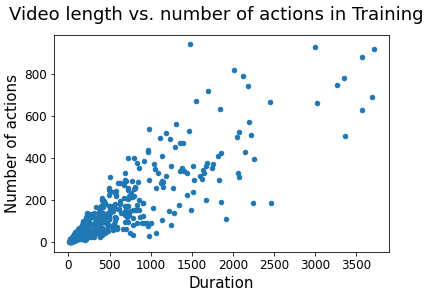
\includegraphics[scale=0.42]{figures/length_vs_actions_Training.png}
%         \end{subfigure}\\
%         \begin{subfigure}[b]{0.475\textwidth}
%             \centering
%             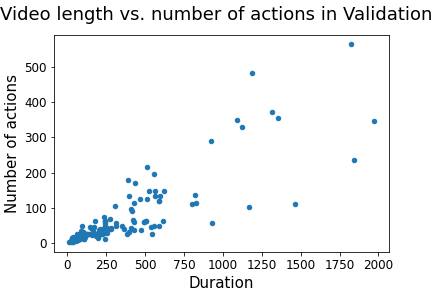
\includegraphics[scale=0.42]{figures/length_vs_actions_Validation.png}
%         \end{subfigure}
%         \caption{Number of action in each video against video length (in seconds)}
%         \label{fig:action-freq-video-length}
%     % \end{minipage}
% \end{figure}

\subsubsection{Video Frame Analysis}
We extract RGB frames from the videos at a sampling rate of 50 FPS. Each frame is identified by participant id, video id, and a start/end frame number. More than half of the total 700 videos in the dataset have less than 25,000 frames.  

Videos in EPIC-KITCHENS-100 have varied length with the longest video of 3708 seconds and shortest video of 10 seconds. 85.7 $\%$ of the videos are shorter than 1000 seconds and 66.0 $\%$ are less than 500 seconds (Appendix A Table \ref{table:train_val_stats}, Figure \ref{fig:duration}). 
%lacking sufficiency in support of longer videos.
% \cite{graphbased2020} mentioned that optimization tends to be slow for longer videos in action recognition tasks. 
We also see that the number of narrations grows roughly linearly with video length (Figure \ref{fig:action-freq-video-length}).  

%[Trim] If need to trim, we can trim on example words%
% The top-10 verb classes with the most number of frames include actions like \textit{grate, wait, prepare, knead, stir}, and \textit{cut}; while those with the least number of frames contain actions like \textit{bend, turn-off, turn-on, take, close}.  and the average length of the action aligns with how people would respond if asked about which action would take longer. It seems that actions involved during cooking take longer than those related to intermediate preparatory steps. 
We compile all training and validation samples of a given verb class and compute the average number of frames for this class (Appendix Figure \ref{fig:avg-frame}). For most verb classes, the average number of frames in each class are roughly the same in both training and validation set, except a few where the validation sets have more frames. We also count the total number of frames for each verb class, summed over all training and validation samples in the class. We notice that such frequency corresponds to the trend of verb-class frequency in the annotations (Appendix A Figure \ref{fig:total-frame}). This indicates that within the dataset, the frequency of the verb class correlates to the amount of visual information in the dataset.

%The dataset also provides bounding-box annotations for each frame, where it only distinguishes between two categories: hands and objects. Only active objects are annotated, so the number of object bounding-boxes in a frame approximates the number of objects that the person interacts with. We compute the average number of hand bounding-boxes appearing in a frame of each verb class. 
%Class with less than 1.5 hand bounding-boxes include actions like \textit{take, put-on, open, pull-down, walk}, and these correspond roughly to human impression on how many hands are needed for performing the action. We also compute the average number of objects bounding boxes in a frame of a given verb class. Verb classes with less than 1.8 object bounding boxes include actions like \textit{open, close, shake, check, fold}, and \textit{drink} (Appendix A Figure \ref{fig:hand-bbox}, \ref{fig:obj-bbox}). 
% \todo[inline]{Would be nice if we can generalize like more avg number of bounding boxes correlates to xx type of action?}
%The average numbers of hand and object bounding boxes for the training and validation sets are mostly equal, despite the validation set misses a few verb classes. Full details can be found in Appendix \ref{appendix:A}.




\subsection{Metrics}
%Frame-wise metrics is most commonly used in segmentation and include accuracy, precision, and recall. However, this group of metrics tends to be influenced more by actions with long duration than by those with short duration \cite{wang2020temporal}. Another problem is that it does not penalize for over-segmentation errors in the model \cite{wang2020temporal, 8099596}. Therefore, we also consider segmental edit distance, which is useful because it reflects out-of-order and over-segmentation errors \cite{ 8099596}. 

We measure our performance based on segmental F1 score, edit score, and frame wise accuracy \cite{8099596}. For each predicted action segment, we calculate its IoU with respect to the corresponding ground truth. If the score is above a threshold $\tau$, then the prediction is considered as a true positive (TP) otherwise a false positive (FP). Over-segmentation is addressed since if more than one correct segments lie within a single true action, only one is labelled as TP and all others are FP.

% We measure three metrics: frame-wise accuracy, segmental edit distance and segmental F1 score.

% Frame-wise metrics is most commonly used in segmentation and include accuracy, precision, and recall. However, this group of metrics tends to be influenced more by actions with long duration than by those with short duration \cite{wang2020temporal}. Another problem is that it does not penalize for over-segmentation errors in the model \cite{wang2020temporal, 8099596}.
% Therefore, we also consider segmental edit distance, which is useful because it reflects out-of-order and over-segmentation errors \cite{ 8099596}. 

% \cite{8099596} also introduces segmental F1 score, which not only penalizes for over-segmentation but also avoids penalizing for minor temporal shifts between the prediction and the ground truth. It also has the advantage of depending on the number of actions instead of their duration. For each predicted action segment, we calculate its IoU with respect to the corresponding ground truth. If the score is above a threshold $\tau$, then the prediction is considered as a true positive (TP) otherwise a false positive (FP). Over-segmentation is addressed since if more than one correct segments lie within a single true action, only one is labelled as TP and all others are FP. Here we consider overlapping thresholds of 10\%, 25\% and 50\%, denoted by F1$@\{10,25,50\}$. 





% We use four methods as our baseline models: both EDTCN \cite{8099596} and MSTCN++ \cite{8953830} use temporal convolution networks to capture long-range dependencies. DTGRM \cite{wang2020temporal} uses multi-level dilated temporal graphs with an auxiliary self-supervised task to help correct wrong temporal relation in videos

\section{Models}

\subsection{Baselines}
We have three baseline models: FC, MS-TCN \cite{9186840}, and DTGRM \cite{wang2020temporal}. 

%%%%%%%%%%%%% excluded opening on baseline section
% both EDTCN \cite{8099596} and MS-TCN++ \cite{9186840} use temporal convolution networks to capture long-range dependencies. \newcite{8099623} proposed a hybrid usage of GRU-based RNN and HMM to refine action alignment. DTGRM \cite{wang2020temporal} uses multi-level dilated temporal graphs with an auxiliary self-supervised task to help correct wrong temporal relation in videos.

\paragraph{FC}
We implement a vanilla 2-layer fully connected neural network that performs frame-wise classification on the input video frames. The inputs are features of dimension 1024 extracted using pretrained I3D \cite{8099985}. 

\paragraph{MS-TCN}
MS-TCN \cite{8953830} is a multi-stage architecture using TCN. The first layer of a single-stage TCN (SS-TCN) adjusts inputs dimension, followed by several dilated 1D temporal convolution layers with dilation factor doubled at each layer. All layers have ReLU activation with the residual connection. MS-TCN stacks multiple SS-TCNs so that each takes initial prediction probabilities from the previous stage and refines it. The overall architecture is trained with the cross entropy classification loss and a truncated mean squared error over the frame-wise log probabilities that penalizes over-segmentation. 

\paragraph{DTGRM}
\newcite{wang2020temporal} proposed DTGRM which refines a predicted result given by the backbone model (e.g. I3D) iteratively. The model stacks $K$ dilated graph convolution layers to perform temporal reasoning across long timescales, where each layer updates the hidden representation of every input frame. To reduce over-segmentation error, an additional self-supervised task is introduced to simulate over-segmentation error by randomly exchanging part of input frames. Both the original and exchanged frame sequences are fed into the model as input, with the output being action class likelihood for two frame sequences as well as exchange likelihood for each frame. 
% Since the model was trained on datasets with relatively shorter videos compared to EPIC-KITCHENS, we plan to trim the videos into overlapping clips of length 15 minutes with fixed fps for consistency.

%%%%%%%%%%%%%%%%%%%%%%%%%%%%%%%%% Tiff short version

% Our main baseline model is MS-TCN \cite{9186840}, which uses temporal convolution networks to capture long-range dependencies.

% \paragraph{MS-TCN}
% MS-TCN \cite{8953830} is a multi-stage architecture using TCN. The first layer of a single-stage TCN (SS-TCN) adjusts inputs dimension, followed by several dilated 1D temporal convolution layers with dilation factor doubled at each layer. All layers have ReLU activation with the residual connection. MS-TCN stacks four SS-TCNs so that each takes initial prediction probabilities from the previous stage and refines it. The overall architecture is trained with the cross entropy classification loss and a truncated mean squared error over the frame-wise log probabilities that penalizes over-segmentation. 

\subsection{Proposed Approach} \label{section:proposed-approach}
% It is relatively difficult for MSTCN to start learning the class of each input feature early: at the beginning, it naturally tries to predict the most frequent verbs in the dataset because of the use of cross-entropy loss. 
% Why Slow-Fast. 
% Following the paper [slow-fast], which proposes a two stream approach, where the fast branch tries to capture motions in the segments and getting a general sense of how objects move in the scene,  
% The intuition is that the objects in view are signature  

% What about your approach is difficult?

% What about your approach is uniquely multimodal?

% What kinds of issues will you likely run into that are caused by it being multimodal? (e.g. the types of things we’ve discussed in class about training, fusion, spurious correlations, etc)

% Can you motivate why those are likely to be issues?

% Do you have thoughts/ideas/preliminary steps on how to mitigate those issues to be successful?

Experiments on baseline models have demonstrated that one major issue with the pre-existing action segmentation methods like MSTCN on EPIC-KITCHENS dataset is to correctly classify the actions of each segment since EPIC-KITCHENS has much more diverse action classes than other datasets \cite{5995444, 10.1145/2493432.2493482, 6909500} that the baselines have evaluated on. Therefore, our proposed method utilizes MSTCN as a backbone model assisted by region of interest visual feature extraction and improves classification with an extra video-text matching component.

\subsubsection{Region of Interest Visual Feature Extraction}
As discussed earlier, one potential problem with the EPIC-KITCHENS dataset is the imbalance in the representation of visual and textual data. While the visual data contains both rich spatial and temporal information, the short verb-noun phrases provide very limited context to build an equally-representative textual space. To account for this imbalance, we assist the video-text embedding by providing visual inputs that aligns with the verb-noun annotations: we extract specific regions in the visual frames that represent actions and/or objects. 

The SlowFast network \cite{feichtenhofer2019slowfast} consists of two streams of feature extractions: the Fast pathway focuses on extracting temporal information across a set of densely sampled frames, while the Slow pathway focuses on representing spatial semantics with high channel capacity and low temporal rate. Moreover, we want to incorporate region of interest (RoI) proposals into the feature extraction procedure such that we extract features of specific objects and actions and discard additional context such as background since textual information lacks additional context. Instead of passing in the full-resolution frame into the SlowFast network, we pass in sub-parts of the frame as proposed by Region Of Interest (RoI) models, thereby extracting object-specific or action-specific visual features. 

\subsubsection{Backbone Model}
We use the original implementation of MSTCN in \newcite{8953830} as the backbone model since experiments on baselines show that it performs relatively well on finding action boundaries. The inputs to the backbone model are the RoI visual features extracted from the SlowFast network. Given the feature vectors $(\mathbf{x}_1,\dots,\mathbf{x}_M)$ of a video, the model outputs an initial segmentation $(\hat{\mathbf{y}}_1,\dots,\hat{\mathbf{y}}_M)$ where $M$ is the number of frames and $\hat{\mathbf{y}}_i$ is the action class label of the predicted verb of frame $i$.


\subsubsection{Video-Text Matching}

Since misclassification is one of the prominent issue in the baseline experiments, our proposed solution utilizes an enriched, pretrained video-text embedding to improve the labeling. We first extracted frame-level and video-level features similarly as in \newcite{miech19howto100m}. 2D features are extracted with the ImageNet pre-trained Resnet-152 \cite{7780459} at the rate of about 1 FPS, and 3D features are extracted with the Kinetics \cite{8099985} pre-trained ResNeXt-101 16-frames model \cite{8578783} to obtain about 0.78 feature per second. Denote the 2D features as $(\mathbf{x}^{2D}_1,\dots,\mathbf{x}^{2D}_{M_{2D}})$ and the 3D features as $(\mathbf{x}^{3D}_1,\dots,\mathbf{x}^{3D}_{M_{3D}})$ where $\mathbf{x}^{2D}_i,\mathbf{x}^{3D}_i\in\mathbb{R}^{2048}$.
Given an initial segmentation result produced by the backbone model $(\hat{\mathbf{y}}_1,\dots,\hat{\mathbf{y}}_M)$, we first find the set of frame indexes corresponding to segment $i$ as $(s_i^{2D})_{i=1}^t$ and $(s_i^{3D})_{i=1}^t$ respectively, where $t$ is the number of segments, then we aggregate the features of one segment using temporal maxpooling and concatenate 2D and 3D features to form a single 4096-dimensional feature vector
\begin{align*}
    \mathbf{v}^{2D}&=maxpool(\{\mathbf{x}_j^{2D}\}_{j\in s_i^{2D}})\\
    \mathbf{v}^{3D}&=maxpool(\{\mathbf{x}_j^{3D}\}_{j\in s_i^{3D}})\\
    \mathbf{v}_i&=concat(\mathbf{v}^{2D},\mathbf{v}^{3D})
\end{align*}
Similar to \newcite{miech19howto100m}, we also use the GoogleNews pre-trained word2vec embedding model to obtain a word embedding $\mathbf{c}_i$ for each verb $i$ (96 $c_i$ if using actions for each action category, $977$ $c_i$ if differentiating among actions within the same action category). We then transform $\mathbf{v}_i,\mathbf{c}_i$ using the learned projection function finetuned on EPIC-KITCHENS $f:\mathbb{R}^{2048}\to\mathbb{R}^d,g:\mathbb{R}^{2048}\to\mathbb{R}^d$ where $d$ is the dimension of the common video-text embedding space. Finally, we perform video-text matching between a segment $\mathbf{v}_i$ and every verb $\mathbf{c}_i$ by computing the cosine similarity score as
\[s(\mathbf{v}_i,\mathbf{c}_j)=\frac{\langle f(\mathbf{v}_i),g(\mathbf{c}_j)\rangle}{\|f(\mathbf{v}_i)\|_2\|g(\mathbf{c}_j)\|_2}\]
which is high when the action $\mathbf{c}_j$ is likely to take place in the segment represented by $\mathbf{v}_i$.

\subsubsection{Improve Video-Text Matching with Cross-Modal Attention}
The above describes a dual encoder model that independently maps text and video to a joint embedding. It has the advantage in scalability as it can results in efficient evaluation during test time. However, as \newcite{miech2021thinking} points out, it has limited accuracy since the simple dot product is unlikely to capture the complex vision-text interactions. Analogous to how human perform video-text retrieval, one solution is to roughly select a few promising candidates then do fine-grained search for the best candidate by paying more \emph{attention} to visual details. Therefore, we adapt the \emph{Fast} and \emph{Slow} models of \newcite{miech2021thinking} in which the \emph{fast} dual encoder quickly eliminates candidates with low relevance while the \emph{slow} cross-attention model improves retrieval performance with grounding. Given an input segment $\mathbf{v}_i$, we perform retrieval by searching for an action class $\mathbf{c}_j$ such that segment $\mathbf{v}_i$ is most likely to decode action class $\mathbf{c}_j$. Specifically, given segment and action class pair $(\mathbf{v}_i, \mathbf{c}_j)$, we compute their similarity by \[
    h(\mathbf{v}_i, \mathbf{c}_j) = \log (p(\mathbf{c}_j|\phi(\mathbf{v}_i);\theta))
\]
where $\phi(\mathbf{v}_i)$ is extracted feature of segment $\mathbf{v}_i$ and $\theta$ is the parameters of the transformer model. To combine results from dual encoder model and cross-attention model, given input segment $\mathbf{v}_i$ and action class set $\mathcal{C}$ containing $K$ action classes. we first obtain a subset of $m$ action classes $\mathcal{C}_m$ (where $m \ll K$) that have the highest score according to the fast dual encoder model. We then retrieve the final top ranked action class by re-ranking the candidates using the cross attention model:
\[
    \mathbf{y}^*_i=\text{argmax}_{\mathbf{c}_j\in \mathcal{C}_m} h(\mathbf{v}_i, \mathbf{c}_j) + \beta s(\mathbf{v}_i,\mathbf{c}_j)
\]
where $\beta$ is a positive hyper-parameter that weights the output scores of the two models. We output $(\mathbf{y}^*_i)_{i\in s_i^{3D}}$ as new labels for segment $i,i\in[t]$.

\subsubsection{Novelty and Challenges}
While most existing action segmentation methods work purely with video input, our approach is the first attempt to action segmentation in the multimodal setting. In particular, we exploits the semantic meaning of the text annotations to improve performance. Moreover, most action segmentation methods evaluate on smaller and simpler datasets, while EPIC-KITCHENS that we attempt is comparably much larger and more complex.

Meanwhile, existing methods aim to learn better temporal relationships among frames that are close together or far away from each other. For example, MSTCN uses dilated convoltuion and MSTCN++ improves with two branches of dilated convolutions each with a different dilation factor; DTGRM contains layers of graphs with nodes spanning neighborhoods of different sizes. These models, by surveying frames across time and learning temporal relationships, aim to differentiate between frames from the same action versus those from different actions. The intuition behind our method, however, is that an action verb, such as \textit{take}, represents a very generic idea that could correspond to a large number of video segments with different contexts that are confounding factors: the specific objects that \textit{take} happens on, other irrelevant objects in the scene, the background of the kitchen, or the way a \textit{take} action takes place. Therefore, if the video-text matching model can make all video segments of \textit{take} clustering around the word \textit{take} in the joint embedding, then it will eliminate the distractions from intraclass variation within the category \textit{take}.

Without extensive training and fine-tuning, when evaluated on recall metrics, R$@\{1,5,10\}$, the projection model gives comparable result as in the original pretrained HowTo100M model on image-text retrieval of the MSR-VTT dataset. However, the retrieval happens between videos and texts of the same batch; if we project all action verbs to the embedding space and rank which verb is the closest to a given video segment, the result is less desirable. Therefore, learning a good joint embedding space will be the biggest challenge of our method, especially given that we pre-tested with segments extracted from a video with ground truth start and end frame. Furthermore, the matching results are likely to be largely dependent on the initial segmentation. If the output from MSTCN is too noisy, which is very likely at the beginning stage of training, the video-text matching model might end up mapping all ambiguous segments, which contain a mix of parts from different actions, to a space that is equidistant away from all word embeddings of the action verbs. A potential solution to this issue may be to train MSTCN for a few epochs for a more stabilized and credible segmentation before adding in the video-text matching model to better guide classification.

We will also attempt to use the more meaningful, full annotation phrase in the form of (verb, noun) pair in the video-text matching. We expect this to create further challenge, one of which is the joint embedding may focus on clustering based on the objects rather than the actions. For example, if we have four segments corresponding to \textit{take apple}, \textit{take banana}, \textit{put-down apple}, \textit{put-down banana}, despite ideally we want \textit{take apple} and \textit{take banana} to be closer, it is possible that \textit{take apple} and \textit{put-down apple} segments are closer since the manipulated objects \textit{apple} and \textit{banana} are more ``visible" in the video. In that way, the video-image matching model will not help with classifying actions. The non-descriptive nature of the annotations makes it difficult to learn a joint embedding space that separates segments of different actions.

% \subsection{Potential Experiment}

\subsubsection{HowTo100M}

Given that the pretrained model does not work well for video-text retrieval on EpicKitchen dataset, we investigate a couple aspects:
\begin{itemize}
    \item Our use of HowTo100M is different from its original use: the model wants to retrieve the corresponding caption for a given video segment, and the caption is usually a descriptive sentence that reflects the video content. The training loss also reflects that there is only one positive within a batch, namely video-text pair $(\mathbf{v}_i, \mathbf{c}_i)$ that share the same index $i$. This is problematic for us since we want all $\mathbf{c}_i$ and all $\mathbf{v}_j$ corresponding to the same action to be close together irrespective of their indices in the batch. 
    
    Therefore, we can try to train with triplet loss that is computed based on the action labels $l \in \{0,\dots,96\}$. In a given batch of size $N$, there is a total of $2N^3$ triplets. 
    The first type of $(i,j,k)$ is $\mathbf{c}_i$, $\mathbf{v}_j$, $\mathbf{c}_k$, where given $\mathbf{v}_j$, $\mathbf{c}_i$ is the positive text, and $\mathbf{c}_k$ is the negative text.
    The second type of $(i,j,k)$ is $\mathbf{c}_i$, $\mathbf{v}_j$, $\mathbf{v}_k$, where given $\mathbf{c}_i$, $\mathbf{v}_j$ is the positive video, and $\mathbf{v}_k$ is the negative video. 
    We need to mask out pairs where 1) $l_i \neq l_j$ 2) $l_i = l_k$ 3) $i == j$.   
    
    \item One hypothesis is that $6144$ is too large of an embedding space for our limited text input. However, how limited is our text input compared to YouCook2? 
    
    \item By looking at the top-10 retrieved texts for a given video of YouCook2, which is also a cooking-based video dataset and whose domain is the closest to ours, we find that the captions are also a set of verbs and nouns, although they are much longer and comprise several actions. In comparison, our segment contains only one action and one pair of verb-noun in the phrase. 
    
    Therefore, another potential experiment is to combine several segments together so that we have a longer caption with multiple action verbs and nouns. In this way, we hope to replicate the YouCook2 results after finetuning.  
\end{itemize}


\section{Results}


% \begin{table*}[t]
% \begin{center}
%     \begin{minipage}[b]{1\textwidth}
% \begin{tabular}{lrrrrrr}
% \toprule
% & \multicolumn{3}{c}{Train} & \multicolumn{3}{c}{Test}\\
% Methods  & Acc & Edit & F1$@\{10,25,50\}$ & Acc & Edit & F1$@\{10,25,50\}$ \\
% \midrule
% FC  & 44.00 & 26.71 & 12.42~~22.64~~19.40 & 34.90 & 18.58 & 17.47~~13.66~~8.04\\
% % EDTCN \cite{8099596} & & & & & & \\
% MS-TCN \cite{8953830} & 43.52 & & & 38.65 & & \\
% % RNN+HMM \cite{8099623} & & & & & & \\
% DTGRM \cite{wang2020temporal} & 52.58 & & & 37.71 & & \\
% \midrule
% Proposed Method (\textit{narration})           & & & & \\
% Proposed Method (\textit{narration+context})           & & & & \\
% \bottomrule
% \end{tabular}
% \caption{Results of baseline models}
% \label{table:results}
% \end{minipage}
% \end{center}
% \end{table*}





\subsection{HowTo100M Experiments} \label{section:howto100m-experiments}
We conducted experiments to evaluate the quality of the video-text joint-embedding learnt after finetuning the HowTo100M model. For a video which is made up from $N$ segments, we use the ground truth start and end frame number, $(s_i,e_i)$, to segment out the $i$-th actions. Following the feature extraction procedure described in Section~\ref{section:video-text-matching}, we extract visual feature $\mathbf{v}_i$ for the $i$-th segment. In order to test what kinds of text input is helpful in building the joint-embedding, we consider two kinds of input in describing the action in a given segment and use the word2vec model mentioned in \ref{section:video-text-matching} to extract the text embeddings: embedding $\mathbf{c}^{verb}_i$ denoting single action verb, and $\mathbf{c}^{narr}_i$ denoting entire narration including verb and noun. 

In Table~\ref{table:howto100m_seg_threshold} and Table~\ref{table:howto100m_label}, the \textit{Label} column shows different $\mathbf{c}{'}_i$ used to calculate the similarity score $s(\mathbf{v}{'}_i, \mathbf{c}{'}_i)$ for video-text retrieval. For 
\textit{Narration}, $\mathbf{c}{'}_i$ is $\mathbf{c}^{narr}_i$; for 
\textit{Verb}, $\mathbf{c}{'}_i = \mathbf{c}^{verb}_i$; for \textit{Verb+Context}, $\mathbf{c}{'}_i = concat(\mathbf{c}^{verb}_{i-1}, \mathbf{c}^{verb}_i)$; for \textit{Narration+Context}, $\mathbf{c}{'}_i = concat(\mathbf{c}^{narr}_{i-1}, \mathbf{c}^{narr}_i)$. We also run experiments on a subset of all segments by filtering out segments that are less than \textit{Segment Threshold}$\times 64$ frames long (in the original 50fps sampling rate). Moreover, in Table~\ref{table:howto100m_visual_seg_threshold}, we vary $\mathbf{v}^{'}_i$ to see the impact of including visual features from neighboring segments. When $l_v = l$, 
$\mathbf{v}^{'}_i = concat(\{\mathbf{v}_j\}_{j\in [i-l\dots i]})$. 

\subsection{MS-TCN Experiments} \label{section:mstcn-experiments}
We selected the best performing HowTo100M joint embedding model and used it after the prediction of MS-TCN to generate the final prediction, as explained in detail in Section~\ref{section:video-text-matching}. We evaluate the trained joint embedding on action segmentation task by using it as a post-processing mechanism on MS-TCN's predicted output. Selecting the two better performing embedding setting, we evaluate our embedding on \textit{Narration} and \textit{Narration + Context} setting. After obtaining the segments' start-end predictions $(s_i,e_i)_{i \in [N']}$, instead of retrieving the closest narration, we retrieve from word embeddings in the form of 
$conat(\mathbf{c}^{pred}_{i-1}, \mathbf{c}_j)$, where $\mathbf{c}^{pred}_{i-1}$ is the narration that is the closest to the $(i-1)$-th segment in the joint-embedding. Moreover, we skip over segments that are predicted as background by MS-TCN. We show results for both retrieval with the original text input $\mathbf{c}_j$ and the text input with context $conat(\mathbf{c}^{pred}_{i-1})$ in Table~\ref{table:results}. 

\begin{table}[b]
\resizebox{\linewidth}{!}{
\begin{minipage}[c]{\linewidth}
\centering
\begin{tabular}{lrrrr}
\toprule
Label & MR & R1 & R5 & R10 \\
\midrule
Verb & \multicolumn{4}{c}{Fail to learn}  \\
Verb+Context & 132 & 0.01 & 0.03 & 0.05\\
Narration & 40 & 0.04 & 0.14 & 0.22 \\
Narration+Context & 16 &  0.19 & 0.49 & 0.66 \\
\bottomrule
\end{tabular}
\caption{Results of Video-Text Retrieval using different types of label}
\label{table:howto100m_label}
\end{minipage}}
\end{table}
% \clearpage
\begin{table*}[h!]
\begin{minipage}[b]{1\textwidth}
\centering
\begin{tabular}{lrrrrrr}
\toprule
% & \multicolumn{3}{c}{Test}\\
Methods  & Acc & Edit & F1$@\{10,25,50\}$ \\
\midrule
FC  & 34.90 & 18.58 & 17.47~~13.66~~8.04\\
% EDTCN \cite{8099596} & & & & & & \\
MS-TCN \cite{8953830} & 38.65 & & \\
% RNN+HMM \cite{8099623} & & & & & & \\
DTGRM \cite{wang2020temporal} & 37.71 & & \\
\midrule
Proposed Method (\textit{narration}) & 20.93 & 24.20 & 2.49 & \\
Proposed Method (\textit{narration+context})& 22.81 & 24.40 & 2.69 & \\
\bottomrule
\end{tabular}
\caption{Results of baseline models}
\label{table:results}
\end{minipage}
~\\
\begin{minipage}[b]{1\textwidth}
\centering
\begin{tabular}{lrrrrr}
\toprule
Label &  Segment Threshold ($l_s$) & MR & R1 & R5 & R10 \\
\midrule
\multirow{3}{*}{Narration} & 0 & 46 & 0.03 & 0.11 & 0.18 \\
 & 1 & 40 & 0.04 & 0.14 & 0.22 \\
 & 3 & 13 & 0.10 & 0.30 & 0.45 \\
\midrule
 & 1 & 132 & 0.01 & 0.03 & 0.05 \\
Verb+Context & 3 & 104 & 0.01 & 0.04 & 0.07 \\
 & 5 & 26 & 0.03 & 0.13 & 0.24\\
\midrule
 & 1 & 6 & 0.19 & 0.49 & 0.66 \\
Narration+Context & 3 & 5 & 0.23 & 0.54 & 0.70 \\
 & 5 & 2 & 0.36 & 0.81 & 0.92 \\
\bottomrule
\end{tabular}
\caption{Results of Video-Text Retrieval using different segment threshold}
\label{table:howto100m_seg_threshold}
\end{minipage}
~\\
\begin{minipage}[b]{1\textwidth}
\centering
% \begin{tabular}{lrrrrr}
\begin{tabular}
{c{0.2\linewidth}  c{0.15\linewidth} c{0.08\linewidth} c{0.08\linewidth}  c{0.08\linewidth}  c{0.08\linewidth}}
\toprule
Visual Context Threshold ($l_v$) & Segment Threshold ($l_s$) & MR & R1 & R5 & R10 \\
\midrule
2 & 0 & 135 & 0.01 & 0.03 & 0.07 \\
3 & 0 & 50 & 0.02 & 0.08 & 0.16 \\
4 & 0 & 26 & 0.03 & 0.16 & 0.27 \\
3 & 1 & 36 & 0.03 & 0.14 & 0.23 \\
3 & 3 & 102 & 0.02 & 0.09 & 0.14 \\
\bottomrule
\end{tabular}
\caption{Results of Video-Text Retrieval using different segment threshold on visual features}
\label{table:howto100m_visual_seg_threshold}
\end{minipage}
\end{table*}

\section{Analysis}
\paragraph{Datasets} 
EPIC-KITCHENS is the largest egocentric dataset. Compared to other egocentric datasets such as GTEA \cite{5995444} and cooking datasets such as 50Salads \cite{10.1145/2493432.2493482} and Breakfast \cite{6909500}, EPIC-KITCHENS contains much longer videos and richer verb classes. In addition, while 50Salads  mostly contains consecutive actions, actions in EPIC-KITCHENS are usually separated by background frames where no action is being performed. These background frames comprise a significant portion of all frames (about 32\%) and affect the performace of baseline models, especially the simpler ones. 

\paragraph{FC}
A 2-layer fully connected network is trained with batch size 16 for 50 epochs. The input frames are down-sampled to 1.25FPS. Since the classification is performed frame-wise and considers no temporal relations, the result is highly fragmental. We further note that the model tends to overfit at an early stage. The poor generalizability is indicated by the relatively low Edit score and Figure \ref{fig:baseline_qualitative}. %TODO: include graph. 

% $26.5\%$ of them were background and $13.5\%$ of them were the wash verb class. %
\paragraph{MSTCN} MSTCN demonstrates its effectiveness in segmenting out the most frequent label classes. The top 5 most frequent labels in the training set in EPIC-KITCHENS are the background, \emph{wash}, \emph{take}, \emph{put}, and \emph{cut} class. We observe that the model assigns one of the most frequent verb classes when it struggles to label the action classes. The result implies that the model is able to memorize the label frequency. One potential way to alleviate this situation is to normalize the frequency through the positional weights supplied to each class label.

EPIC-KITCHENS is more complex than the benchmark datasets in many aspects, such as longer video durations and thus more actions involved. We accounted for this increase in complexity by using 15-layer single-stage TCNs rather than the 10-layer ones which are claimed to achieve optimal performance in the original experiment \cite{8953830}. Our experiment shows that there is an improvement in when using a more complex model.

\paragraph{DTGRM} The DTGRM model builds off MSTCN by adding an additional fine-tuning component that refines segmentation around the boundaries. Similar to MSTCN, DTGRM is able to output reasonable segmentation results. \ref{fig:baseline_qualitative} shows that one of its improvements from MSTCN is its capability in clearly segmenting out smaller segments, which proves the effectiveness of the additional fine-tuning component even on a more complex dataset like EPIC-KITCHENS. However, we also notice that DTGRM tend to over-segment on videos with fewer segments.

DTGRM also suffers from the label class imbalance problem. Similar to MSTCN, it labels majority of the segments as the most frequent vocabulary classes in the training set. With the weighted loss, DTGRM is able to predict a wider variety of labels. However, the classification accuracy is not as high as in the original experiment \cite{wang2020temporal}. This is reasonable given the richer vocabulary classes available in EPIC-KITCHENS.

Due to limitations on hardware, we are not able to expand the number of layers in the DTGRM model. To accommodate this, we sampled the feature inputs for every 10 frames of input to decrease input size. The more complex, sub-sampled DTGRM improved the over-segmentation issue in the original DTGRM by avoiding overly short segmentation under a sub-sampled setting.

\paragraph{Comparison Between Models}
The FC model is able to quickly gain performance at the start of training, but the performance also saturates early on. This indicates that the dataset and task requires a more complex model to learn. We observed that both the performance of MSTCN and DTGRM suffered from unbalanced verb class labels. This is a problem introduced by the EPIC-KITCHEN dataset, increasing the difficulty of the action segmentation task. 

DTGRM has shown better performance in segmenting short action instance. However, on long action instances, DTGRM does not perform as well as MSTCN as the predictions of DTGRM tends to be heavily over-segmented.
%Dataset having unequal distribution of labels
%Learning the labels instead of learning the actual task
%Interesting point is that it learns backgrounds well, which could imply it knows "when" an action is taking place, just don't know "what" it is, so it guesses the most frequent action?%

\begin{figure*}[ht!]
\begin{center}
    \begin{minipage}[b]{1\textwidth}
        \begin{subfigure}[b]{0.475\textwidth}
            \centering
            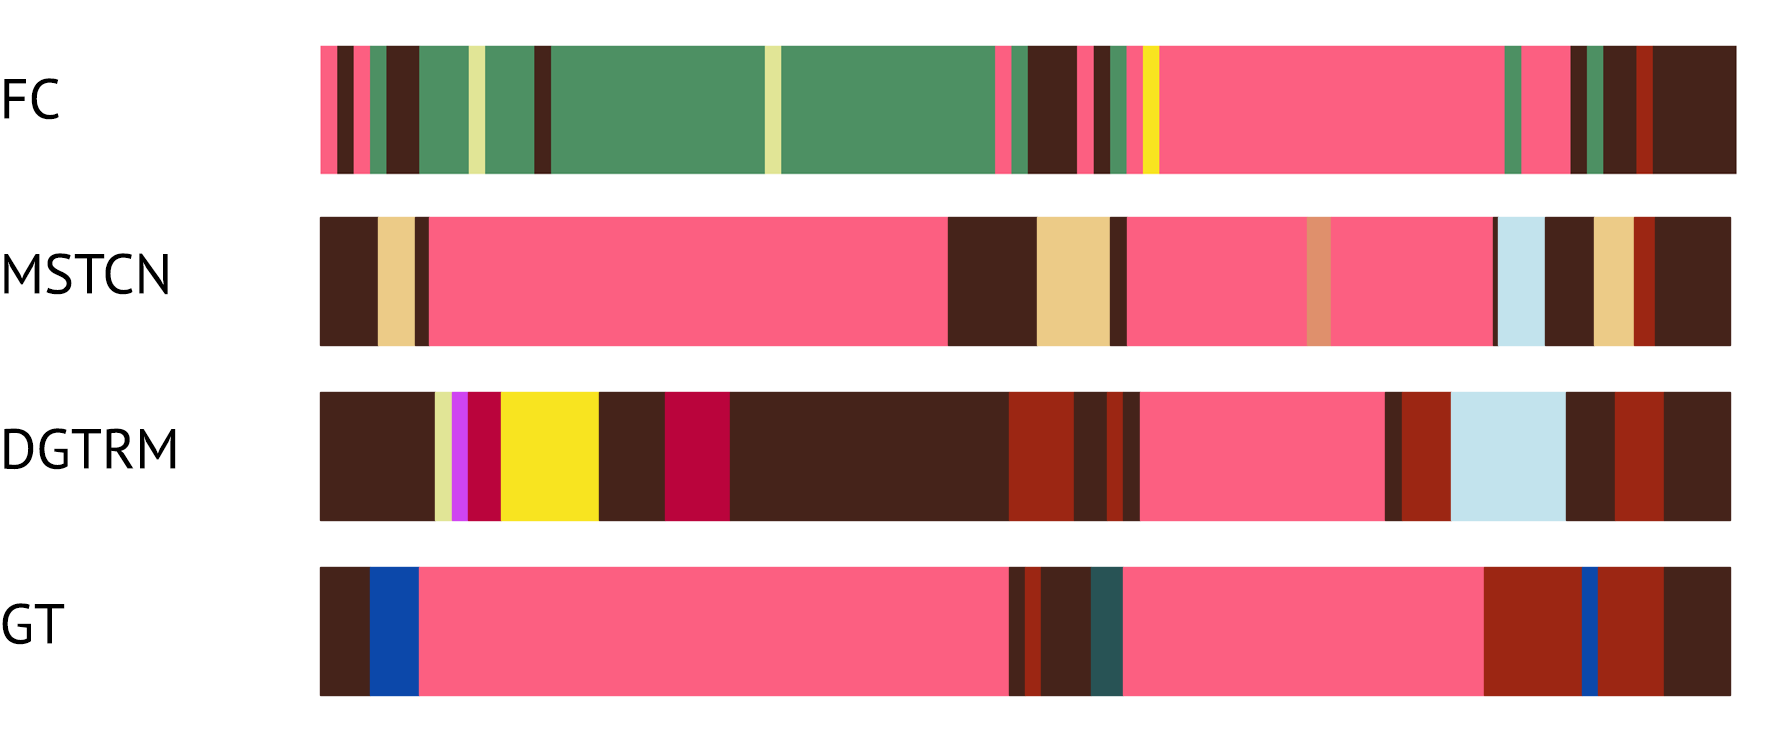
\includegraphics[scale=0.12]{figures/P26_39-comparison.png}
            \caption{P26\_39}
            \label{fig:2639}
        \end{subfigure}\quad
        \begin{subfigure}[b]{0.475\textwidth}
            \centering
            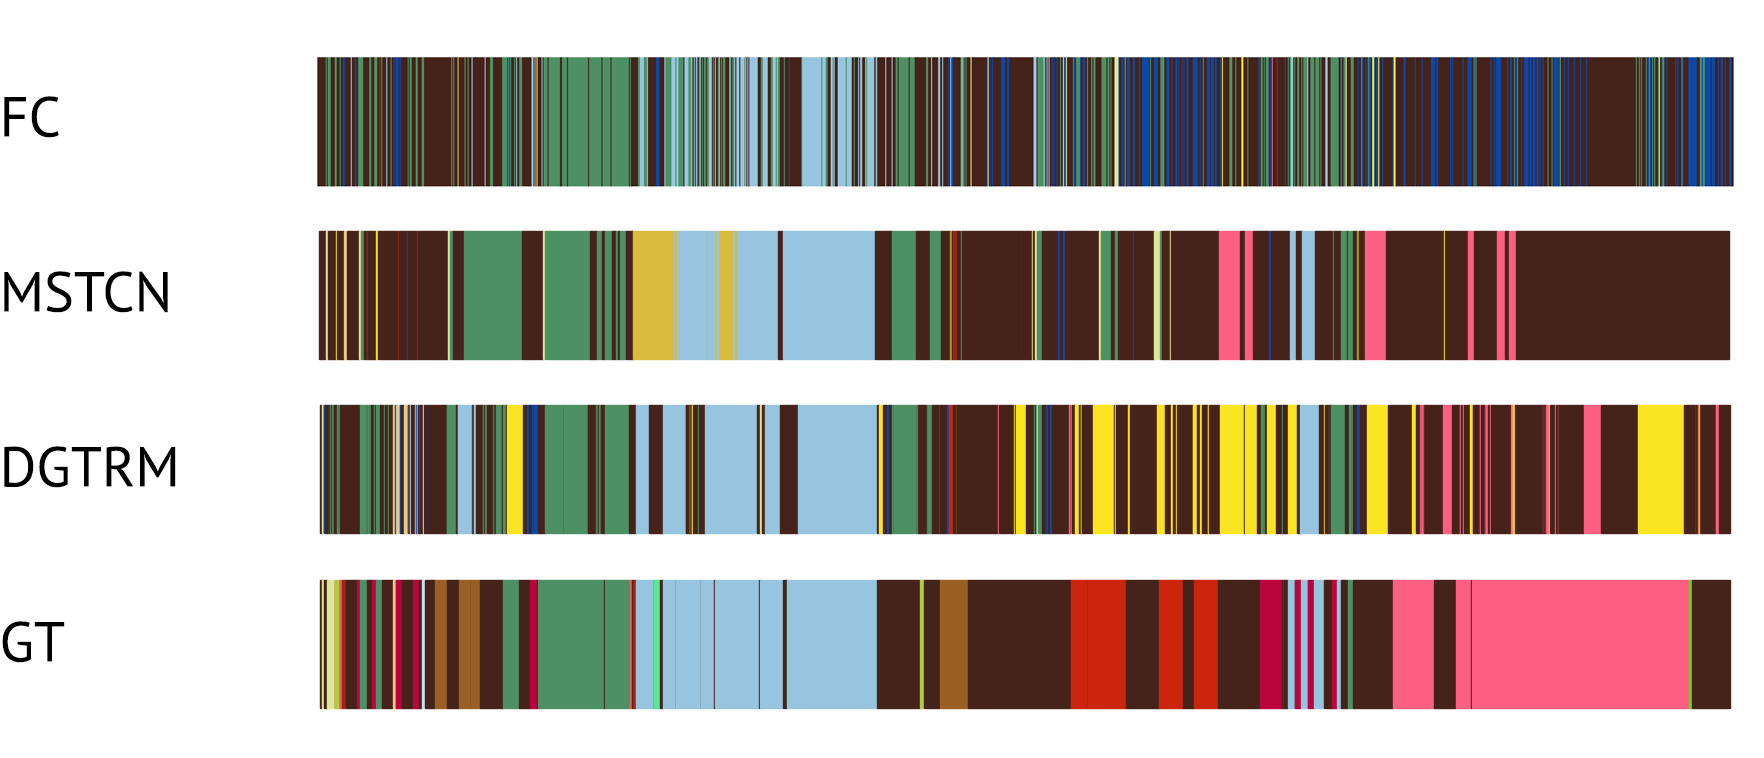
\includegraphics[scale=0.12]{figures/P16_04-comparison.png}
            \caption{P16\_04}
            \label{fig:1604}
        \end{subfigure}
        \caption{Qualitative results of two videos across all models.}
        \label{fig:baseline_qualitative}
    \end{minipage}
\end{center}
\end{figure*}

\paragraph{Metrics} 
We experimented with two variants of loss function: cross-entropy loss with and without weighting. Since background frames comprise a sizable portion, one phenomenon we observe during training is that models tend to classify most of the frames as background, at least in the first few iterations. Down-weighting background classes can mitigate this issue, but inconsistency still exists between the loss function and metrics we used, since classifying frames as the most common verb class (e.g. background, \emph{wash}) can quickly increase frame-wise accuracy until some threshold (usually the percentage of these common verb class). Edit score is a better reflection of the fragmentation issue. Models like MSTCN that incorporate temporal information tend to have higher Edit score than simpler models such as FC.  

\subsection{Analysis of Text-Video Retrieval} 
With the aim of building more robust joint embedding space, we experimented Howto100m retrieval model on EPIC-KITCHENS dataset under different settings, as explained in Section~\ref{section:howto100m-experiments}. From Table \ref{table:howto100m_label}, we see a strong positive correlation between richness of text and performance of retrieval. With plain verbs as label, the retrieval result is orders of magnitudes worse than other settings. By adding more textual information to just verb, we see improvements in median-rank of true label and recall scores in both \textit{Narration} (current narration) and \textit{Narration+Context} (previous and current narrations). The reason that using noun helps is more obvious: for verbs that cannot be easily visualized or doesn't correspond to a single action (e.g. \textit{take}), the less ambiguous object can narrow down the search space for appropriate verbs. 

In addition to text input, length of segments also affects performance (see Table \ref{table:howto100m_seg_threshold}). By only considering segments that contain more than \textit{Segment Threshold} number of features, we found that the longer the segments, the better the retrieval performance. Because the model uses maxpooling across video features from the same segment, the final video feature for the segment contains the most eminent features within the segment. However, since ground truth and video feature are not perfectly aligned (videos are downsampled before feature extraction), there are inevitable noise at the boundary of segments. Thus the shorter the segment, the noisier the video feature.   

% \subsection{Ablations and Their Implications}
\subsection{Analysis of post-MSTCN Text-Video Retrieval} 


\subsubsection{Video length}
Variation of video length for EPIC-KITCHENS dataset is much higher than that of other datasets. The maximum video length is more than 1 hour while average is only 9 minute. To determine how video length affects performance of models, we divided the whole dataset into long videos that are longer than 10 minutes and short videos that are shorter than 10 minutes.  

\subsubsection{Vocabulary size}
EPIC-KITCHENS contains a total of 97 verb classes, which is much more than that of 50Salads and Breakfast, which contain 17 and 48 verb classes respectively. To see if richer verb class will affect the performance of the baseline models that are originally proposed for 50Salads and Breakfast, we select a subset from 97 verb classes containing 54 verb classes with higher correlation to cooking. The remaining verb classes are labeled as background. 
% The training and testing result on the subset is shown in Table \ref{}.

% TODO: include table/graph

\subsection{Qualitative Analysis and Examples}
% This section should likely contain a table of examples demonstrating how the current approach succeeds/fails.

From \ref{fig:var_baseline} we can see that it is very challenging for FC to get the class label correctly, as it predicts the most common verb ``wash" (olive-green) instead of the ground truth ``mix" (hot pink). For videos with a few number of long segments, DGTRM tends to over-segment. In \ref{fig:mstcn_joint} we see that the joint embedding trained with \textit{Narration+Context} gives a slightly better classification result than one trained only with \textit{Narration}, suggesting richness in textual modality is key.



% \subsection{Analysis of SlowFast Visual Feature} \label{section:visual-feature-analysis}
% 
\begin{table*}[t]
\begin{center}
    \begin{minipage}[b]{1\textwidth}
    \centering
\begin{tabular}{lrrrr}
\toprule
  & verb-top-1-acc & verb-top-5-acc & noun-top-1-acc & noun-top-5-acc \\
\midrule
SlowFast (original) & 52.98 & 84.05 & 38.27 & 63.99 \\
\midrule
SlowAlign  & 52.26 & 83.84 & 38.42 & 63.59 \\
FastAlign & 25.94 & 70.59 & 9.87 & 26.46 \\
SlowAlign + Slow & 51.76 & 83.31 & 37.35 & 62.30 \\
FastAlign + Fast & 52.03 & 83.53 & 37.85 & 62.70 \\
\bottomrule
\end{tabular}
\caption{Results of applying RoiAlign at different places of the SlowFast network.}
\label{table:roi-results}
\end{minipage}
\end{center}
\end{table*}


In addition to using text to improve action segmentation performance, we also experiment with ways to extract visual features that could give better performance than the original I3D features. Since text-retrieval componenet did not improve the MSTCN prediction, we experimented without the component. In order to extract better visual features, we decide to use the SlowFast network \cite{feichtenhofer2019slowfast} for feature extraction, because it contains two pathways: the Slow and the Fast pathway.
% focuses on extracting temporal information across a set of densely sampled frames, while the Slow pathway focuses on representing spatial semantics with high channel capacity and low temporal rate. 
Our intuition was that information on changes in the scene, captured by the Fast pathway operating on a set of densely sampled frames, and contents in the scene, encoded by the Slow pathway outputting activations with a large number of channels, are both important to recognizing the action and differentiating between neighboring actions. 

We plan to use region of interest (RoI) proposals of the frames, which are fed into RoiAlign after the SlowFast ResNet backbone. Our motivation is that by excluding the distracting information in the context of the video, focusing on the manipulated objects that are near the hand regions will help with identifying the action, since the text information lacks context; moreover, we assume that changes in how the objects are handled indicate the action performed. 

% \subsubsection{Region of Interest Visual Feature Extraction}

% The SlowFast network \cite{feichtenhofer2019slowfast} consists of two streams of feature extractions: the Fast pathway focuses on extracting temporal information across a set of densely sampled frames, while the Slow pathway focuses on representing spatial semantics with high channel capacity and low temporal rate. Moreover, we want to incorporate region of interest (RoI) proposals into the feature extraction procedure such that we extract features of specific objects and actions and discard additional context such as background since textual information lacks such context. Instead of passing in the full-resolution frame into the SlowFast network, we pass in sub-parts of the frame as proposed by Region Of Interest (RoI) models, thereby extracting object-specific or action-specific visual features. 

% Section 5 details results of our multi-modal approach to the action segmentation task on the EPIC-KITCHENS dataset. To this end, we are interested in analyzing how might changes to one modality affect this multi-modal approach. In an egocentric visual frame, an action often takes place near ones hand and acted upon the object of interest. Inspired by the available hand-object bounding box annotations in EPIC-KITCHENS, we want to see if attending to the hand and object regions assists in the action segmentation task.

% \paragraph{Roi Alignment}
% Our visual feature extractor backbone, SlowFast ~\cite{feichtenhofer2019slowfast}, consists of two pathways. The fast pathway extracts features at a lower temporal rate, capturing higher temporal resolution. The slow pathway consists of higher temporal rate and larger number of channels, indicating richer spatial representation of the frames. We hypothesize that attending to hand-object regions in either the spatial dimension, the temporal dimension, or both can assist in learning visual features that are more suitable for action segmentation tasks. To test this, we utilize the RoiAlignment component to extract areas of interest and extract such features at the output of the pathways in the SlowFast model. SlowFast consists of two unique pathways, we run experiments on all possible combinations of the pathways to evaluate its affect.
In order to determine the quality of the features before passing into MS-TCN, we use performance on action-recognition, the original task described in \citet*{feichtenhofer2019slowfast} but performed on EPIC-KITCHENS segments, as an indicator. Table~\ref{table:roi-results} presents the noun and verb accuracy of different modifications made to the original SlowFast network. 
We first tried to pass the activations from the Fast pathway before the prediction head into RoiAlign, since Fast pathway has much higher sampling rate; the results is shown in the \textit{FastAlign} row. Similarly, \textit{SlowAlign} corresponds to passing activations from the Slow pathway into RoiAlign. \textit{SlowAlign + Slow} shows results of preserving the activations from both pathways but adding an additional branch of output after performing RoiAlign on activations of the Slow pathway, similar idea for \textit{FastAlign + Fast}. 

% \begin{table*}[t]
% \begin{center}
%     \begin{minipage}[b]{1\textwidth}
%     \centering
% \begin{tabular}{lrrrr}
% \toprule
%   & verb-top-1-acc & verb-top-5-acc & noun-top-1-acc & noun-top-5-acc \\
% \midrule
% SlowFast (original) & 52.98 & 84.05 & 38.27 & 63.99 \\
% \midrule
% SlowAlign  & 52.26 & 83.84 & 38.42 & 63.59 \\
% FastAlign & 25.94 & 70.59 & 9.87 & 26.46 \\
% SlowAlign + Slow & 51.76 & 83.31 & 37.35 & 62.30 \\
% FastAlign + Fast & 52.03 & 83.53 & 37.85 & 62.70 \\
% \bottomrule
% \end{tabular}
% \caption{Results of applying RoiAlign at different places of the SlowFast network.}
% \label{table:roi-results}
% \end{minipage}
% \end{center}
% \end{table*}

Poor performance of \textit{SlowAlign} shows that the slow pathway, which contains rich spatial information due to its large channel size, needs full image information, and applying RoIAlign limits its representation significantly. Moreover, similar performances among the other model variations indices that RoiAlign does not provide better representation, and one reason could be that although context in images are not the actively manipulated objects, to determine an action like “open”, changes in the surrounding between frames carry useful information, such as changes in the position of an object relative to the background. 
% We then feed the SlowFast features into MSTCN, but the performance does not improve; details are provided in Appendix. 



\section{Conclusion}
We presented a multi-modal approach to the action segmentation task. Given the difficulty of the action segmentation task and the EPIC-KITCHENS dataset, we want to produce better prediction by post-processing the baseline model's prediction with a trained visual-textual joint embedding. The baseline model follows a multi-stage temporal convolution architecture, and the joint embedding is trained with max-margin ranking loss. Although our experiments show that the proposed methodology does not improve the prediction, we identified potential caveats through analysis of textual and visual information. We also experimented with ways to extract better visual features using SlowFast network, which can be find in Appendix~\ref{section:visual-feature-analysis}, but even though features from SlowFast network work well on action recognition, feeding them into MS-TCN does not improve baseline performance. Similarly, the video-text retrieval model works well with well-trimmed segments but not so when fed with noisy visual features, so in the future, we would like to investigate more about how visual and text input interact across time, since the additional temporal dimension results in most of the complexity in our experiments.  

\newpage
% Please use 
\bibliographystyle{acl_natbib}
\bibliography{references}

\clearpage

\begin{appendices}


\section{Data Analysis}
\label{appendix:A}
\begin{minipage}{1\textwidth}
    In this section, we present the full details of our data analysis.
\end{minipage}
\begin{table}[ht!]
\begin{minipage}{1\textwidth}
\begin{center}
{\small
\begin{tabular}{lrrrrrrrr}
\toprule
& \multicolumn{4}{c}{Training} & \multicolumn{4}{c}{Validation}\\
~ & Max. & Min. & Avg. & Std. & Max. & Min. & Avg. & Std. \\
\midrule
Verb class frequency & 14848 & 73 & 1314 & 2829 & 1937 & 71 & 191 & 398\\
Noun class frequency & 3617 & 178 & 724 & 655 & 430 & 25 & 108 & 92\\
Sentence length & 77 & 3 & 15.1 & 6.3 & 71 & 3 & 14.8 & 6.0\\
Actions per video & 940 & 1 & 136 & 168 & 564 & 3 & 70 & 93\\
Frames per verb class & 2129212 & 20165 & 225170 & 408408 & 407425 & 2702 & 42016 & 76950 \\
Video length & 3708 & 10 & 543 & 645 & 1969 & 11 & 344 & 377 \\
\bottomrule
\end{tabular}}
\caption{Statistics of EPIC-KITCHENS-100 training and validation set}
\label{table:train_val_stats}
\end{center}
\end{minipage}
\end{table}

\begin{figure}[hp]
    \begin{minipage}{1\textwidth}
    \centering
        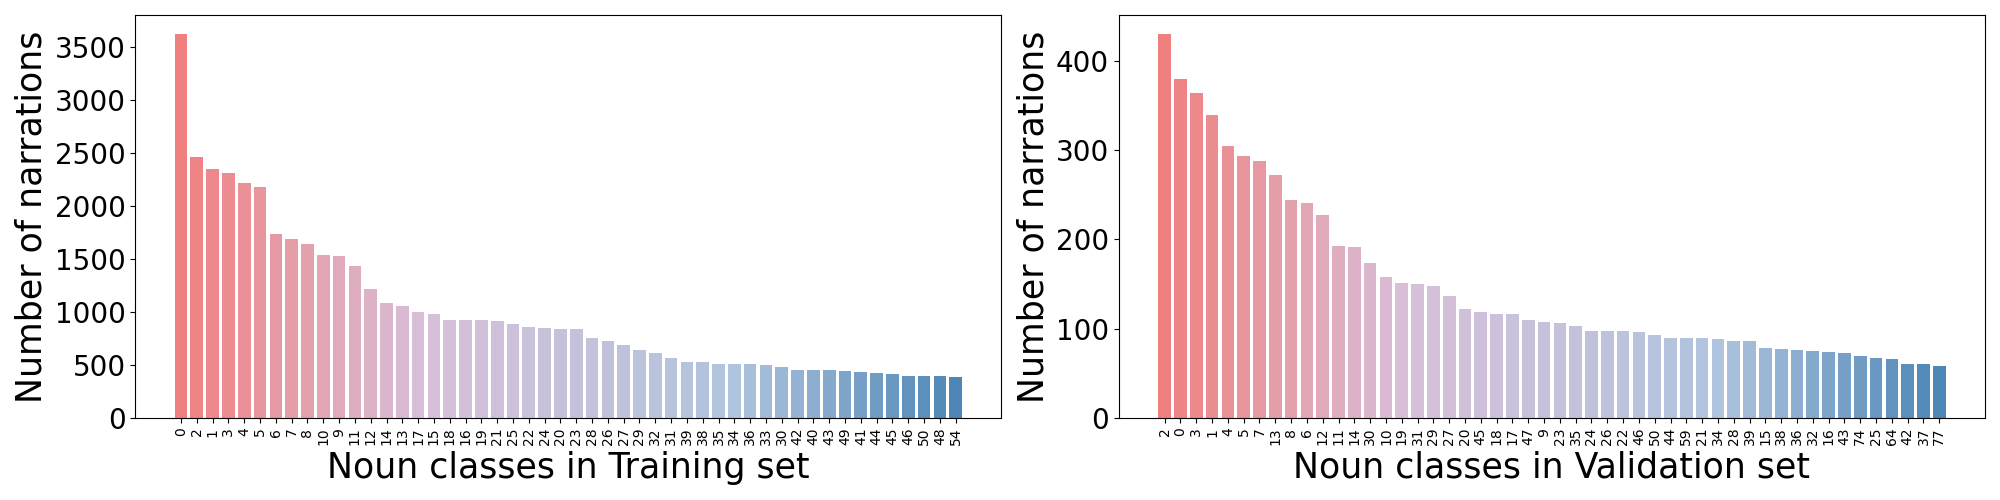
\includegraphics[scale=0.3]{figures/noun_count.png}
    \caption{Frequency distribution of 50 most frequent noun classes in training and validation set}
    \label{fig:noun-freq}
    \end{minipage}
\end{figure}
\begin{figure}[htp!]
    \begin{minipage}{1\textwidth}
        \begin{center}
            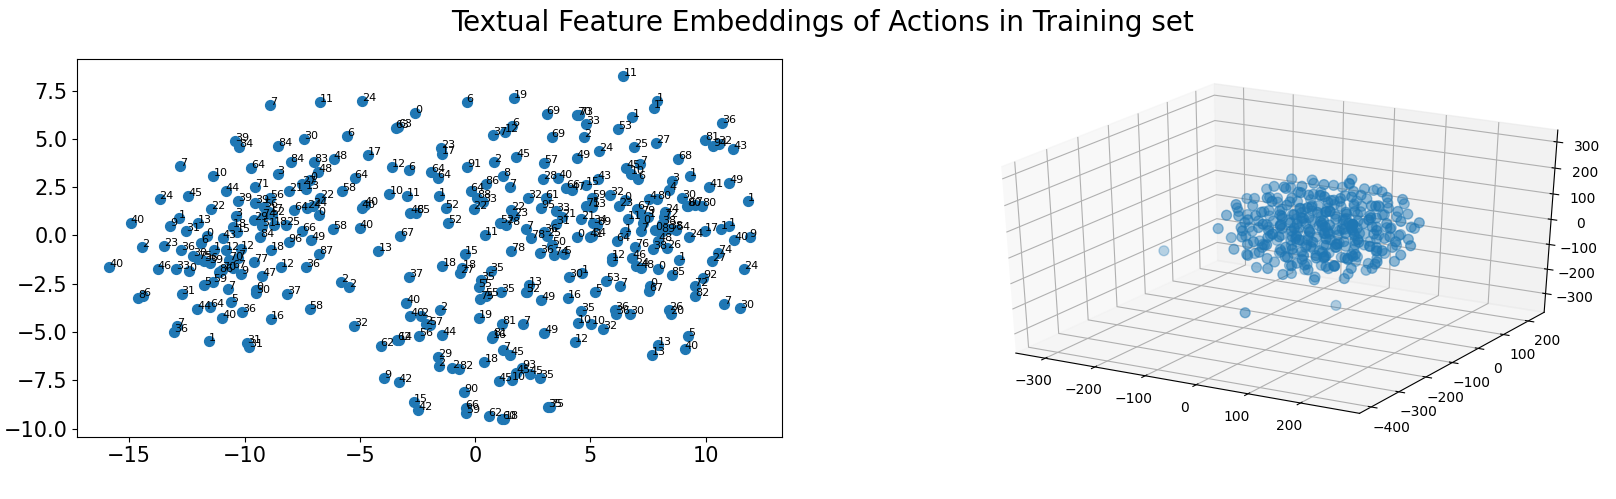
\includegraphics[scale=0.36]{figures/Actions_embeddings_Training.png}
            \\
            \vspace{5mm}
            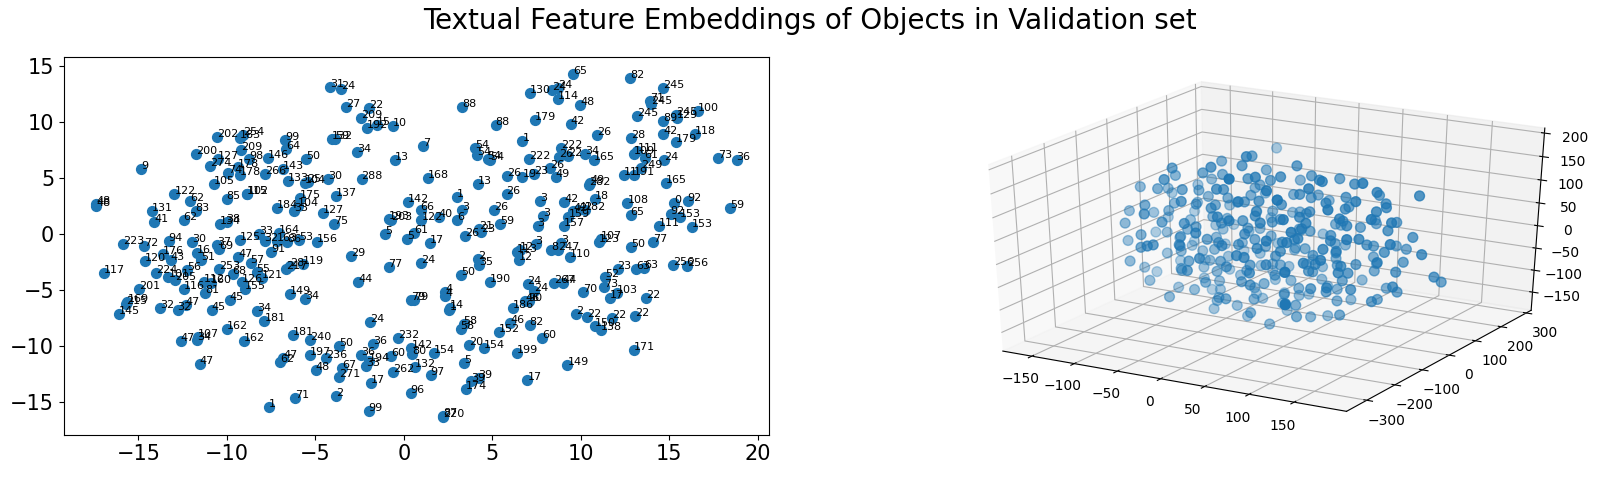
\includegraphics[scale=0.36]{figures/Objects_embeddings_Validation.png}
            \caption{Example of visualizing feature embeddings of verb and noun classes in 2D and 3D space}
            \label{fig:embedding}
        \end{center}
    \end{minipage}
\end{figure}
\clearpage

\begin{figure}[ht!]
    \begin{minipage}[b]{1\textwidth}
        \begin{subfigure}[b]{0.475\textwidth}
            \centering
            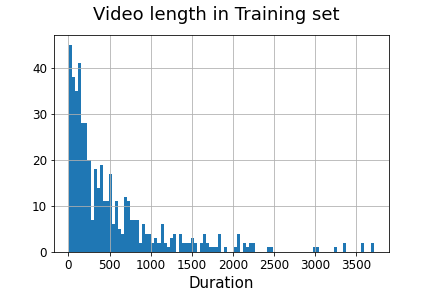
\includegraphics[scale=0.4]{figures/video_length_Training.png}
        \end{subfigure}
        \begin{subfigure}[b]{0.475\textwidth}
            \centering
            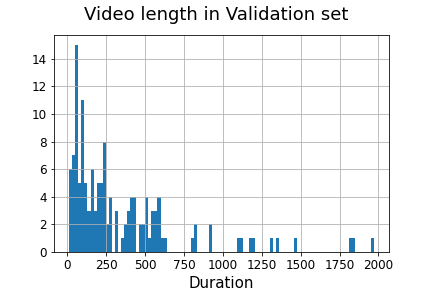
\includegraphics[scale=0.4]{figures/video_length_Validation.png}
        \end{subfigure}
        \caption{Distribution of video length (in seconds)}
        \label{fig:duration}
    \end{minipage}
\end{figure}

\begin{figure}[htp!]
    \begin{minipage}[b]{1\textwidth}
        \centering
        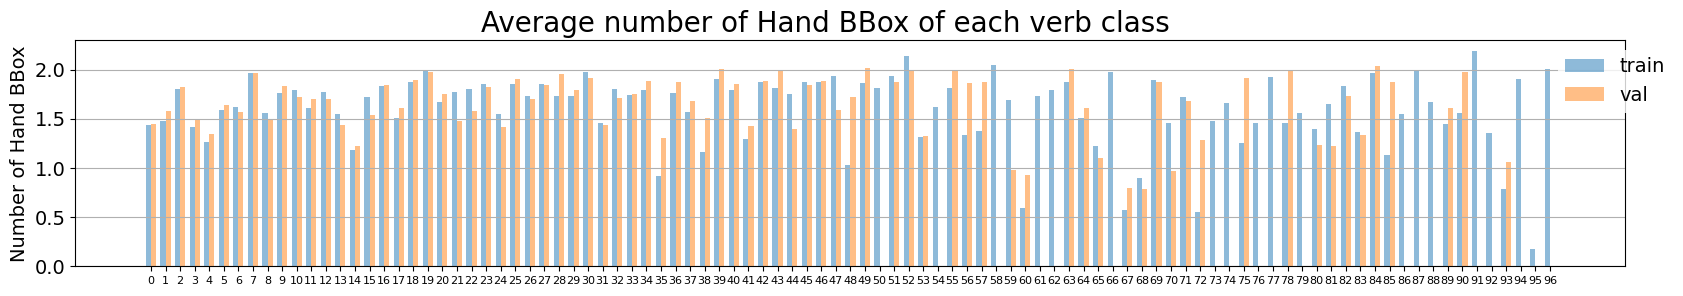
\includegraphics[scale=0.38]{figures/avg_number_Hand_bbox_verb_class.png}
        \caption{Average number of hand bounding-boxes in each frame of given verb class}
        \label{fig:hand-bbox}
    \end{minipage}
\end{figure}

\begin{figure}[htp!]
    \begin{minipage}[b]{1\textwidth}
        \centering
        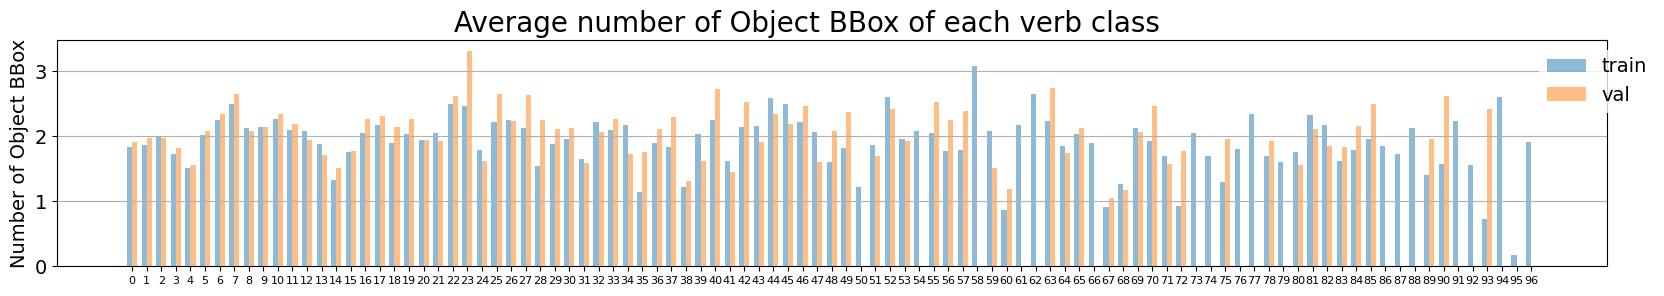
\includegraphics[scale=0.38]{figures/avg_number_Object_bbox_verb_class.png}
        \caption{Average number of object bounding-boxes in each frame of given verb class}
        \label{fig:obj-bbox}
    \end{minipage}
\end{figure}

\begin{figure}[htp!]
    \begin{minipage}[b]{1\textwidth}
        \centering
        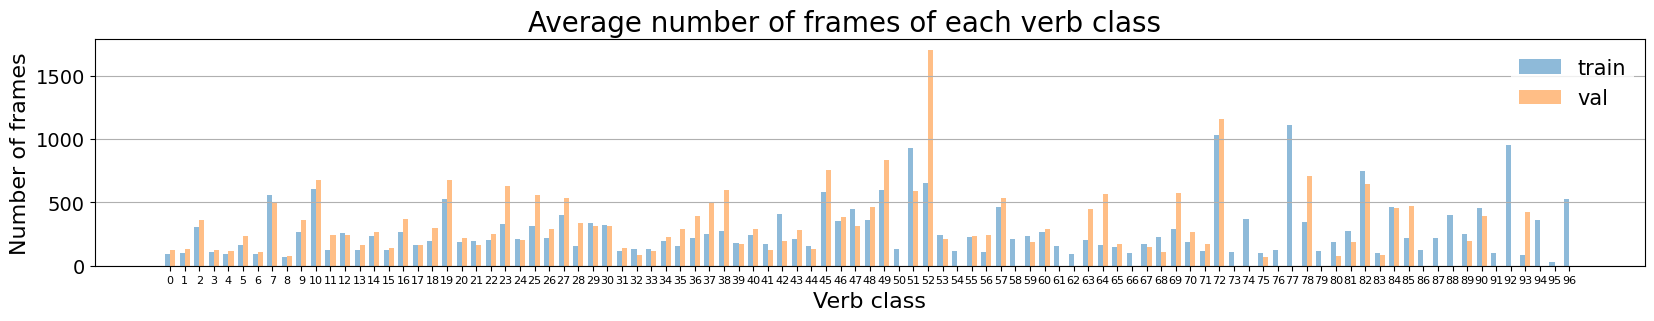
\includegraphics[scale=0.38]{figures/avg_number_frames_verb_class.png}
        \caption{Average number of frames in a narration of a given verb class in training and validation set}
        \label{fig:avg-frame}
    \end{minipage}
\end{figure}

% \begin{figure}[htp!]
% \begin{minipage}[b]{1\textwidth}
%     \begin{minipage}[b]{0.475\textwidth}
%         \begin{subfigure}[b]{0.475\textwidth}
%             \centering
%             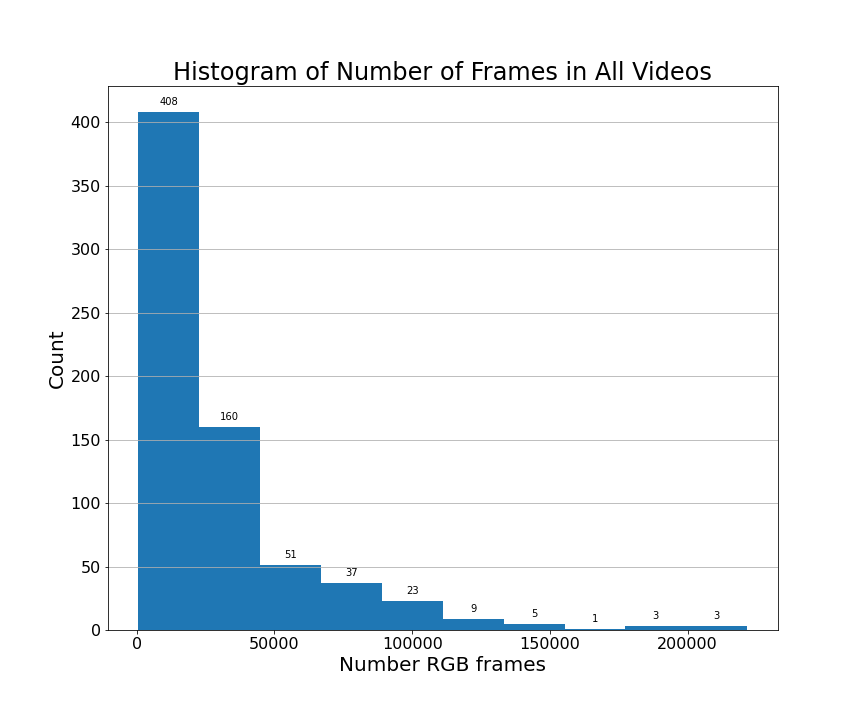
\includegraphics[scale=0.28]{figures/histogram_num_frame_videos.png}
        % \end{subfigure}
        % \begin{subfigure}[b]{0.475\textwidth}
        %     \centering
        %     \includegraphics[scale=0.3]{figures/avg_number_frames_verb_class_4.png}
        % \end{subfigure}
    %     \caption{Distribution of number of frames in each video}
    %     \label{fig:frame-video}
    % \end{minipage}
    % \hfill
    % \begin{minipage}[b]{0.475\textwidth}
    %     \begin{subfigure}[b]{0.475\textwidth}
    %         \centering
    %         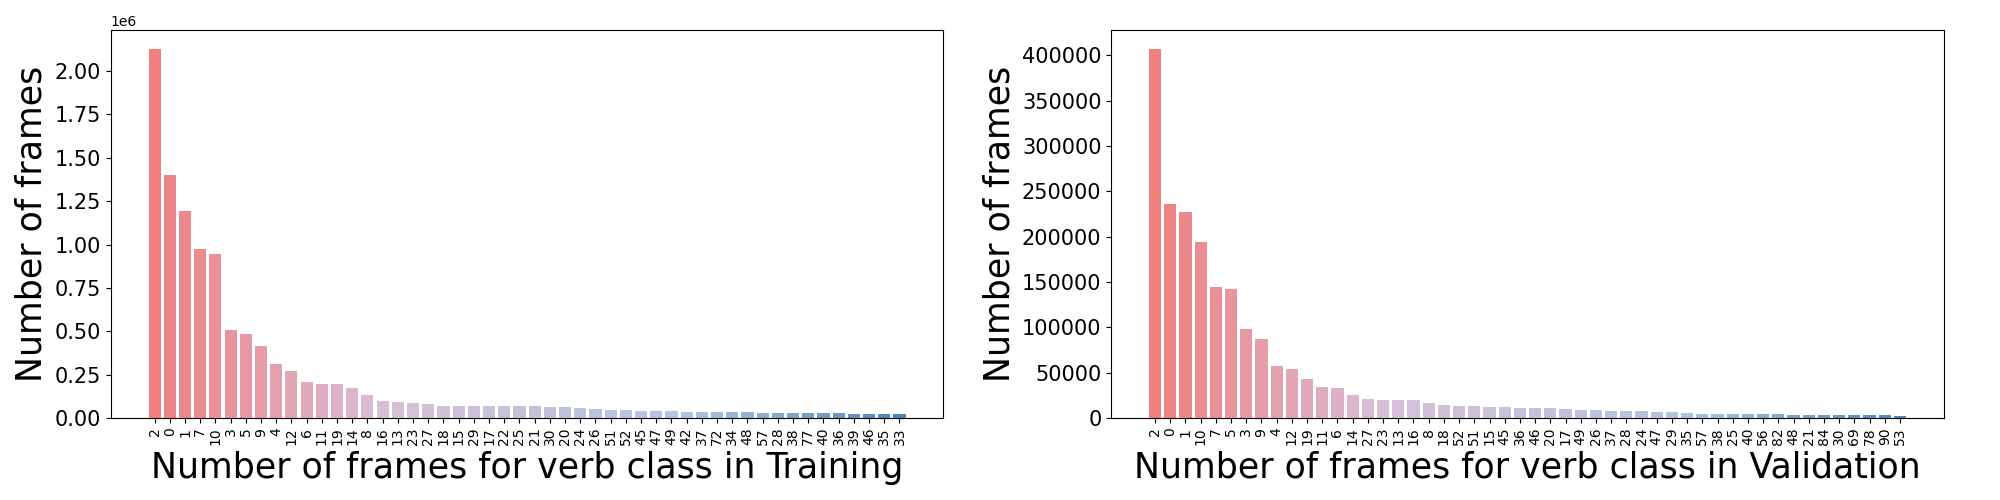
\includegraphics[scale=0.15]{figures/total_frame_word.png}
        % \end{subfigure}
        % \begin{subfigure}[b]{0.475\textwidth}
        %     \centering
        %     \includegraphics[scale=0.3]{figures/avg_number_frames_verb_class_4.png}
        % \end{subfigure}
%         \caption{Distribution of number of frames in each video}
%         \label{fig:total-frame}
%     \end{minipage}
% \end{minipage}
% \end{figure}

% \begin{figure}[htp!]
%     \begin{minipage}[b]{1\textwidth}
%         \begin{subfigure}[b]{0.475\textwidth}
%             \centering
%             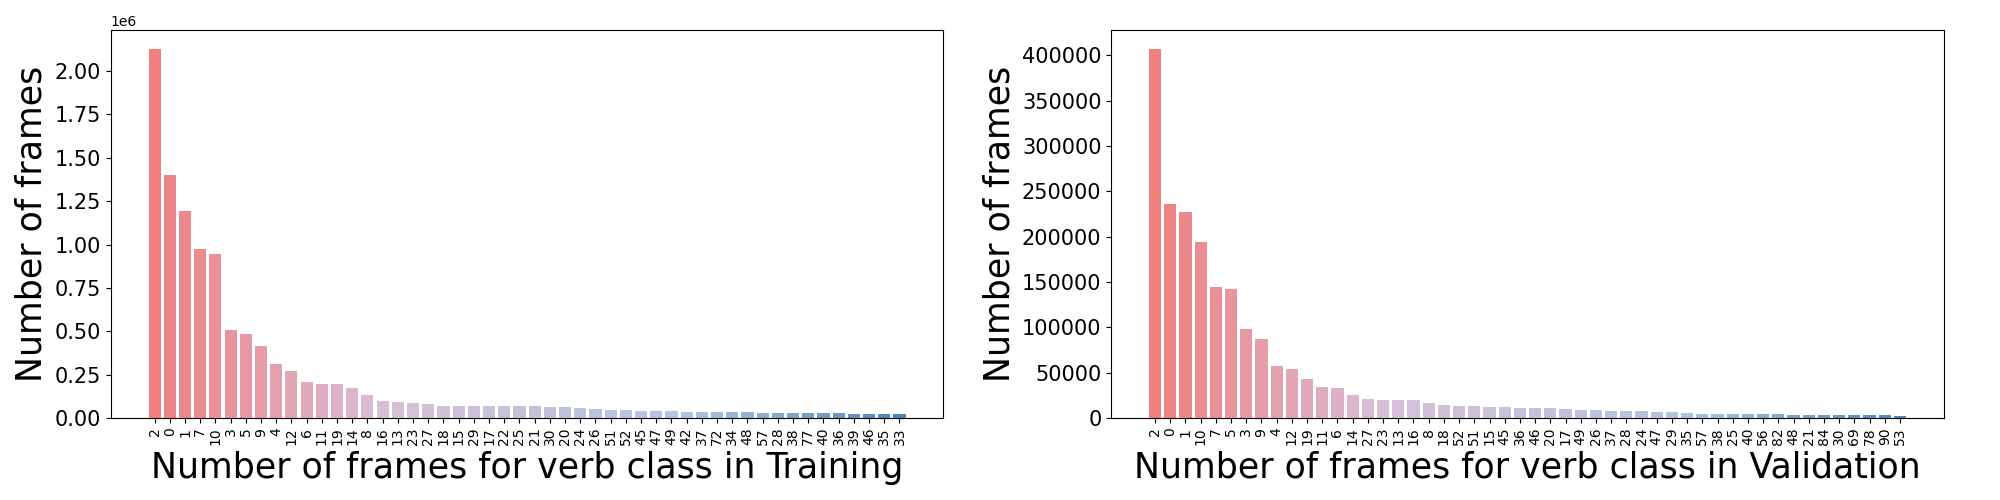
\includegraphics[scale=0.1]{figures/total_frame_word.png}
        % \end{subfigure}
        % \begin{subfigure}[b]{0.475\textwidth}
        %     \centering
        %     \includegraphics[scale=0.3]{figures/avg_number_frames_verb_class_4.png}
        % \end{subfigure}
%         \caption{Histogram of the number of frames in a video}
%         \label{fig:total-frame}
%     \end{minipage}
% \end{figure}

\begin{figure}[htp!]
\begin{minipage}[b]{1\textwidth}
    \centering
    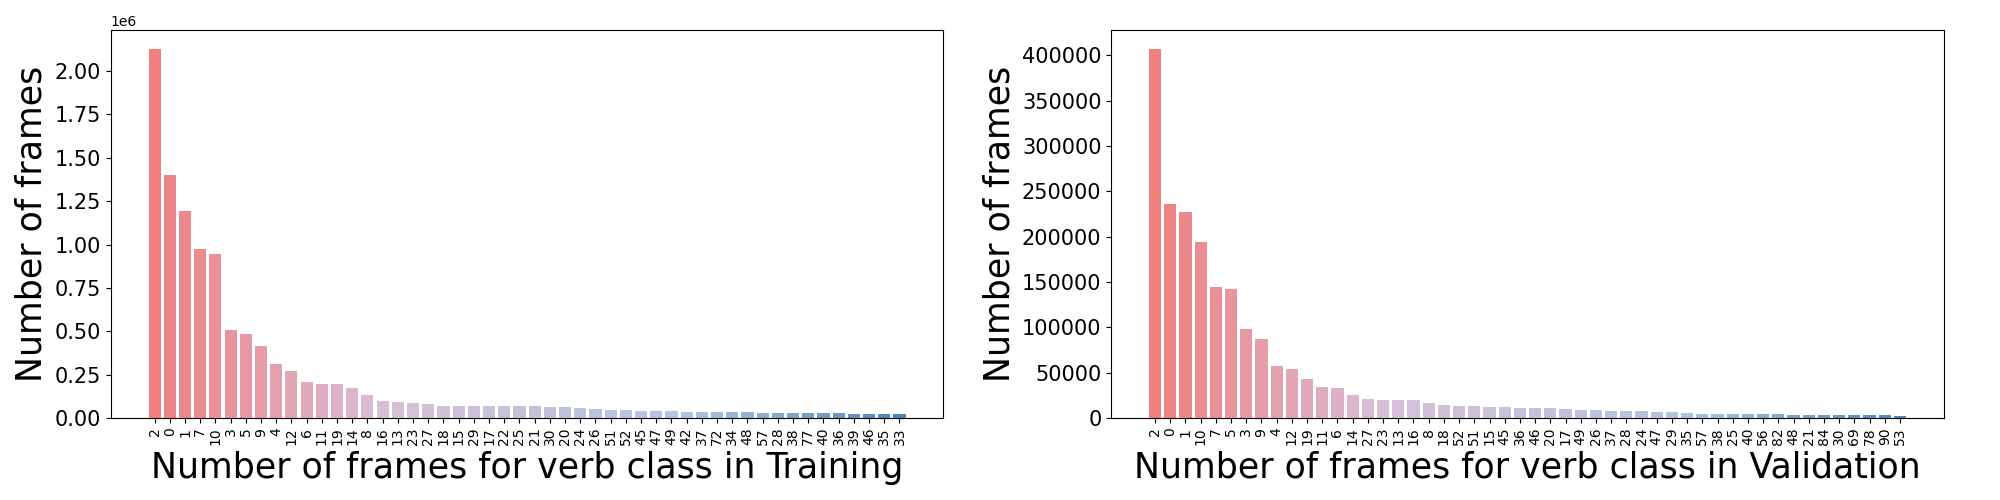
\includegraphics[scale=0.31]{figures/total_frame_word.png}
    \caption{Distribution of number of frames in each video}
    \label{fig:total-frame}
\end{minipage}
\end{figure}

\clearpage

\begin{figure}[t]
    \centering
    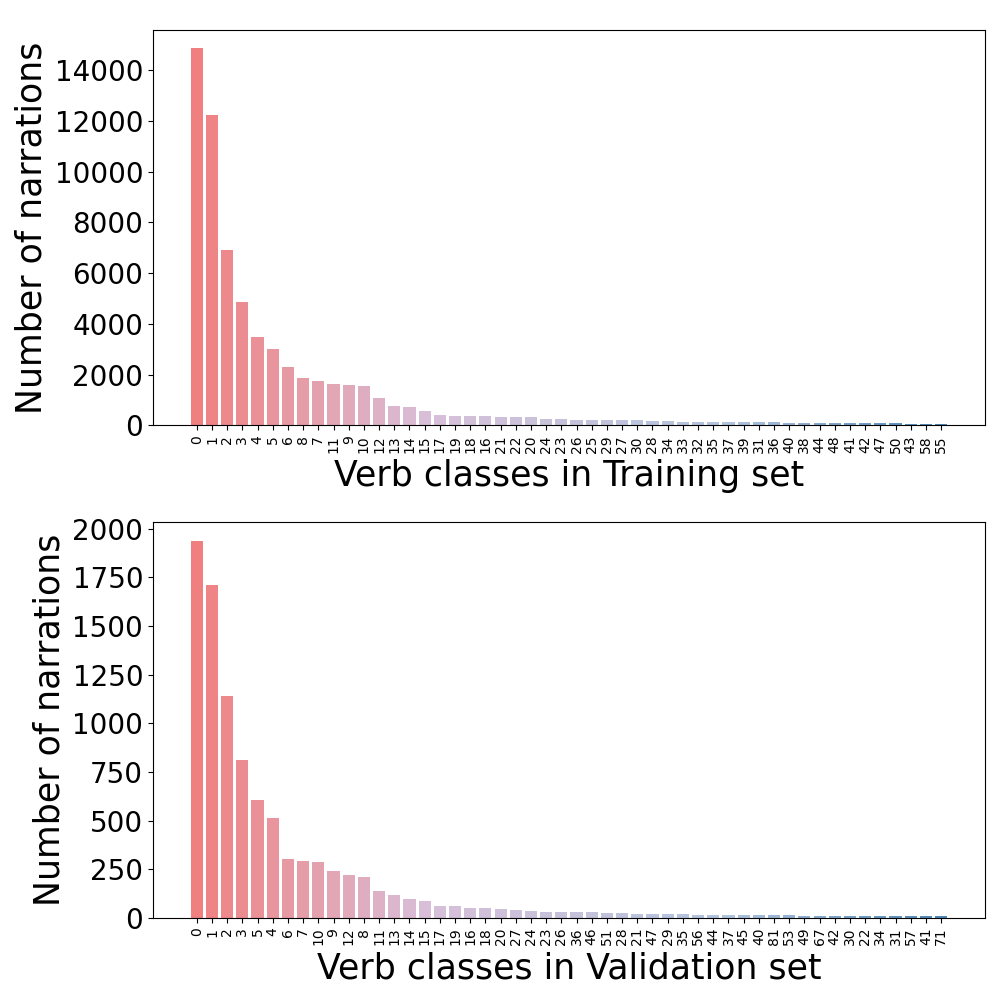
\includegraphics[scale=0.25]{figures/verb_count.png}
    \caption{Frequency distribution of 50 most frequent verb class in training and validation set}
    \label{fig:verb_freq}
\end{figure}

% \subsubsection{Running MSTCN with SlowFast Features} \label{appendix:slowfast}
% We slide 

\begin{figure}[t!]
    % \begin{minipage}[b]{1\textwidth}
        \begin{subfigure}[b]{0.475\textwidth}
            \centering
            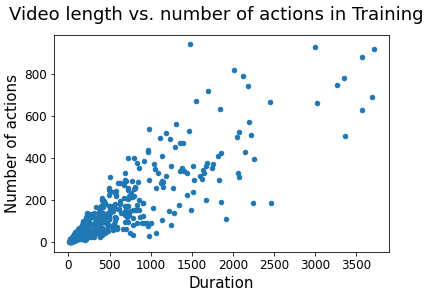
\includegraphics[scale=0.42]{figures/length_vs_actions_Training.png}
        \end{subfigure}\\
        \begin{subfigure}[b]{0.475\textwidth}
            \centering
            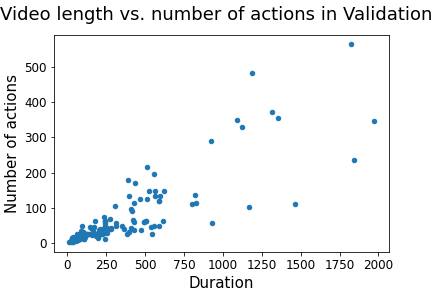
\includegraphics[scale=0.42]{figures/length_vs_actions_Validation.png}
        \end{subfigure}
        \caption{Number of action in each video against video length (in seconds)}
        \label{fig:action-freq-video-length}
    % \end{minipage}
\end{figure}


\subsubsection{Improve Video-Text Matching with Cross-Modal Attention}
The above describes a dual encoder model that independently maps text and video to a joint embedding. It has the advantage in scalability as it can results in efficient evaluation during test time. However, as \newcite{miech2021thinking} points out, it has limited accuracy since the simple dot product is unlikely to capture the complex vision-text interactions. Analogous to how human perform video-text retrieval, one solution is to roughly select a few promising candidates then do fine-grained search for the best candidate by paying more \emph{attention} to visual details. Therefore, we adapt the \emph{Fast} and \emph{Slow} models of \newcite{miech2021thinking} in which the \emph{fast} dual encoder quickly eliminates candidates with low relevance while the \emph{slow} cross-attention model improves retrieval performance with grounding. Given an input segment $\mathbf{v}_i$, we perform retrieval by searching for an action class $\mathbf{c}_j$ such that segment $\mathbf{v}_i$ is most likely to match action class based on the joitnn embedding $\mathbf{c}_j$. Specifically, given segment and action class pair $(\mathbf{v}_i, \mathbf{c}_j)$, we compute their similarity by \[
    h(\mathbf{v}_i, \mathbf{c}_j) = \log (p(\mathbf{c}_j|\phi(\mathbf{v}_i);\theta))
\]
where $\phi(\mathbf{v}_i)$ is extracted feature of segment $\mathbf{v}_i$ and $\theta$ is the parameters of the transformer model. To combine results from dual encoder model and cross-attention model, given input segment $\mathbf{v}_i$ and action class set $\mathcal{C}$ containing $K$ action classes. we first obtain a subset of $m$ action classes $\mathcal{C}_m$ (where $m \ll K$) that have the highest score according to the fast dual encoder model. We then retrieve the final top ranked action class by re-ranking the candidates using the cross attention model:
\[
    \mathbf{y}^*_i=\text{argmax}_{\mathbf{c}_j\in \mathcal{C}_m} h(\mathbf{v}_i, \mathbf{c}_j) + \beta s(\mathbf{v}_i,\mathbf{c}_j)
\]
where $\beta$ is a positive hyper-parameter that weights the output scores of the two models. We output $(\hat{\mathbf{y}}^*_{i,c})$ as the classification probability of frame $i$ as action $c$ based on the similarity score and $(\mathbf{y}^*_i)_{i\in s_i^{3D}}$ as new labels for segment $i,i\in[t]$.


\section{SlowFast Visual Feature} 
\label{section:visual-feature-analysis}

\begin{table*}[t]
\begin{center}
    \begin{minipage}[b]{1\textwidth}
    \centering
\begin{tabular}{lrrrr}
\toprule
  & verb-top-1-acc & verb-top-5-acc & noun-top-1-acc & noun-top-5-acc \\
\midrule
SlowFast (original) & 52.98 & 84.05 & 38.27 & 63.99 \\
\midrule
SlowAlign  & 52.26 & 83.84 & 38.42 & 63.59 \\
FastAlign & 25.94 & 70.59 & 9.87 & 26.46 \\
SlowAlign + Slow & 51.76 & 83.31 & 37.35 & 62.30 \\
FastAlign + Fast & 52.03 & 83.53 & 37.85 & 62.70 \\
\bottomrule
\end{tabular}
\caption{Results of applying RoiAlign at different places of the SlowFast network.}
\label{table:roi-results}
\end{minipage}
\end{center}
\end{table*}


In addition to using text to improve action segmentation performance, we also experiment with ways to extract visual features that could give better performance than the original I3D features. Since text-retrieval componenet did not improve the MSTCN prediction, we experimented without the component. In order to extract better visual features, we decide to use the SlowFast network \cite{feichtenhofer2019slowfast} for feature extraction, because it contains two pathways: the Slow and the Fast pathway.
% focuses on extracting temporal information across a set of densely sampled frames, while the Slow pathway focuses on representing spatial semantics with high channel capacity and low temporal rate. 
Our intuition was that information on changes in the scene, captured by the Fast pathway operating on a set of densely sampled frames, and contents in the scene, encoded by the Slow pathway outputting activations with a large number of channels, are both important to recognizing the action and differentiating between neighboring actions. 

We plan to use region of interest (RoI) proposals of the frames, which are fed into RoiAlign after the SlowFast ResNet backbone. Our motivation is that by excluding the distracting information in the context of the video, focusing on the manipulated objects that are near the hand regions will help with identifying the action, since the text information lacks context; moreover, we assume that changes in how the objects are handled indicate the action performed. 

% \subsubsection{Region of Interest Visual Feature Extraction}

% The SlowFast network \cite{feichtenhofer2019slowfast} consists of two streams of feature extractions: the Fast pathway focuses on extracting temporal information across a set of densely sampled frames, while the Slow pathway focuses on representing spatial semantics with high channel capacity and low temporal rate. Moreover, we want to incorporate region of interest (RoI) proposals into the feature extraction procedure such that we extract features of specific objects and actions and discard additional context such as background since textual information lacks such context. Instead of passing in the full-resolution frame into the SlowFast network, we pass in sub-parts of the frame as proposed by Region Of Interest (RoI) models, thereby extracting object-specific or action-specific visual features. 

% Section 5 details results of our multi-modal approach to the action segmentation task on the EPIC-KITCHENS dataset. To this end, we are interested in analyzing how might changes to one modality affect this multi-modal approach. In an egocentric visual frame, an action often takes place near ones hand and acted upon the object of interest. Inspired by the available hand-object bounding box annotations in EPIC-KITCHENS, we want to see if attending to the hand and object regions assists in the action segmentation task.

% \paragraph{Roi Alignment}
% Our visual feature extractor backbone, SlowFast ~\cite{feichtenhofer2019slowfast}, consists of two pathways. The fast pathway extracts features at a lower temporal rate, capturing higher temporal resolution. The slow pathway consists of higher temporal rate and larger number of channels, indicating richer spatial representation of the frames. We hypothesize that attending to hand-object regions in either the spatial dimension, the temporal dimension, or both can assist in learning visual features that are more suitable for action segmentation tasks. To test this, we utilize the RoiAlignment component to extract areas of interest and extract such features at the output of the pathways in the SlowFast model. SlowFast consists of two unique pathways, we run experiments on all possible combinations of the pathways to evaluate its affect.
In order to determine the quality of the features before passing into MS-TCN, we use performance on action-recognition, the original task described in \citet*{feichtenhofer2019slowfast} but performed on EPIC-KITCHENS segments, as an indicator. Table~\ref{table:roi-results} presents the noun and verb accuracy of different modifications made to the original SlowFast network. 
We first tried to pass the activations from the Fast pathway before the prediction head into RoiAlign, since Fast pathway has much higher sampling rate; the results is shown in the \textit{FastAlign} row. Similarly, \textit{SlowAlign} corresponds to passing activations from the Slow pathway into RoiAlign. \textit{SlowAlign + Slow} shows results of preserving the activations from both pathways but adding an additional branch of output after performing RoiAlign on activations of the Slow pathway, similar idea for \textit{FastAlign + Fast}. 

% \begin{table*}[t]
% \begin{center}
%     \begin{minipage}[b]{1\textwidth}
%     \centering
% \begin{tabular}{lrrrr}
% \toprule
%   & verb-top-1-acc & verb-top-5-acc & noun-top-1-acc & noun-top-5-acc \\
% \midrule
% SlowFast (original) & 52.98 & 84.05 & 38.27 & 63.99 \\
% \midrule
% SlowAlign  & 52.26 & 83.84 & 38.42 & 63.59 \\
% FastAlign & 25.94 & 70.59 & 9.87 & 26.46 \\
% SlowAlign + Slow & 51.76 & 83.31 & 37.35 & 62.30 \\
% FastAlign + Fast & 52.03 & 83.53 & 37.85 & 62.70 \\
% \bottomrule
% \end{tabular}
% \caption{Results of applying RoiAlign at different places of the SlowFast network.}
% \label{table:roi-results}
% \end{minipage}
% \end{center}
% \end{table*}

Poor performance of \textit{SlowAlign} shows that the slow pathway, which contains rich spatial information due to its large channel size, needs full image information, and applying RoIAlign limits its representation significantly. Moreover, similar performances among the other model variations indices that RoiAlign does not provide better representation, and one reason could be that although context in images are not the actively manipulated objects, to determine an action like “open”, changes in the surrounding between frames carry useful information, such as changes in the position of an object relative to the background. 
% We then feed the SlowFast features into MSTCN, but the performance does not improve; details are provided in Appendix. 


\end{appendices}


\end{document}
